\refstepcounter{chapter}
\addcontentsline{toc}{chapter}{Operation of the Machine}

\section{Function Testing / Trial Run}

After setting up the machine and connecting it to the power supply, a function test must be performed.

\vspace{.3cm}

\noindent This section describes machine-specific manual operations. The operation of the control is only explained \textbf{briefly}; detailed instructions can be found in the CNC 432/10-Graphics operating manual.

\begin{itemize}
    \item Turn on the main switch on the control cabinet and wait until the \textbf{Power-On Diagnosis} appears on the screen to identify hardware errors. If no error is found, the screen displays the \textbf{Manual Mode} screen.
    
    \item Unlock all \textbf{Emergency Stop} buttons by turning them to the right.
    
    \item Press the \textbf{Hydraulics} button \raisebox{-0.4\height}{
\includegraphics[height=20pt]{hydraulics_button.jpg}} and then press the \textbf{CLEAR} button. Repeat within 5 seconds.
    
    \item While holding the \textbf{Hydraulics} button, press the \textbf{CLEAR} button to delete error messages.
    
    \item Move the reference points of the individual axes according to the CNC 432/Graphics manual.
    
    \item Press the \textbf{TEACH IN} button.
    
    \item Enter the spindle speed under address \textbf{"S"}, following the CNC 432/10-Graphics manual (e.g., 160 min\(^{-1}\) → \texttt{S 160}) and press the \textbf{ENTER} key.
    
    \item Press the \textbf{START} button \raisebox{-0.4\height}{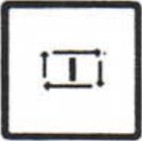
\includegraphics[height=20pt]{start_button.jpg}}. The gearbox engages.
\end{itemize}

\notebox{NOTE}{The working spindle will not rotate until the rotation direction is entered. \enquote{M3} = Clockwise, \enquote{M4} = Counterclockwise.}

\subsection{Entering Spindle Rotation Direction}
\begin{itemize}
    \item Press the \textbf{TEACH IN} button.
    \item Enter the rotation direction under address \textbf{"M"} according to the CNC 432/10-Graphics manual.
    \item Press the \textbf{ENTER} key and the \raisebox{-0.4\height}{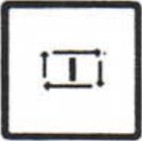
\includegraphics[height=20pt]{start_button.jpg}} button.
\end{itemize}

\notebox{NOTE}{The working spindle rotates according to the entered direction. If the command does not execute correctly, contact MAHO service.}

\subsection{Stopping the Working Spindle via Command \textbf{"M5"}}
\begin{itemize}
    \item Press the \textbf{TEACH IN} button.
    \item Enter the stop command \textbf{"M5"} according to the CNC 432/10-Graphics manual.
    \item Press the \textbf{ENTER} key and the \raisebox{-0.4\height}{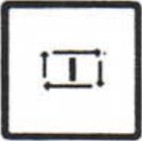
\includegraphics[height=20pt]{start_button.jpg}} button. The working spindle stops.
\end{itemize}

\newpage

\subsection{Stopping with Function Key}

\begin{itemize}
    \item Press the \raisebox{-0.4\height}{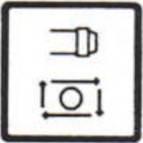
\includegraphics[height=20pt]{stop_button.jpg}} button (feed and rotation stop immediately). If the \raisebox{-0.4\height}{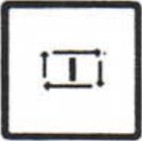
\includegraphics[height=20pt]{start_button.jpg}} button is pressed afterward, the working spindle will restart.
\end{itemize}

\subsection{Shutting Down the System}
The entire system is shut down using the \textbf{main switch} on the control cabinet.

\subsection{Shutting Down via Emergency Stop Button}
The machine can be stopped in any operating state by pressing an \textbf{Emergency Stop (NOT-AUS)} button.

\vspace{.3cm}

\noindent Emergency stop buttons are located on the machine control panel,on the right side of the control cabinet and on the handheld control unit.

\subsection{Releasing the Emergency Stop Button}

\notebox{WARNING}{Before unlocking, the cause of the malfunction must be resolved.}

\begin{itemize}
    \item Turn the affected Emergency Stop button to the right to release it.
    \item Restart the machine.
\end{itemize}

\subsection{Emergency Stop Limits on Machine Slides}
If the software limit fails, a mechanical switch with two cams takes over the Emergency Stop function.  
The affected slide will brake, and an alarm will be displayed on the screen.

\subsection{Restarting After an Emergency Stop}
Restarting after an Emergency Stop follows the instructions on Sheet 3.15-2.

\section{Manual Spindle Speed Selection}

\setcounter{section}{3}
\setcounter{page}{2}

In case of a failure of the automatic speed selection, the spindle speed can be manually adjusted as follows:

\begin{itemize}
    \item Insert a \textbf{12 mm hex key} into the gear shift shafts (1), (3), and (5) of the main gearbox and rotate left or right until the corresponding color markers appear in the openings (2), (4), and (6), according to the speed selection table.
\end{itemize}

\begin{figure}[h]
    \centering
    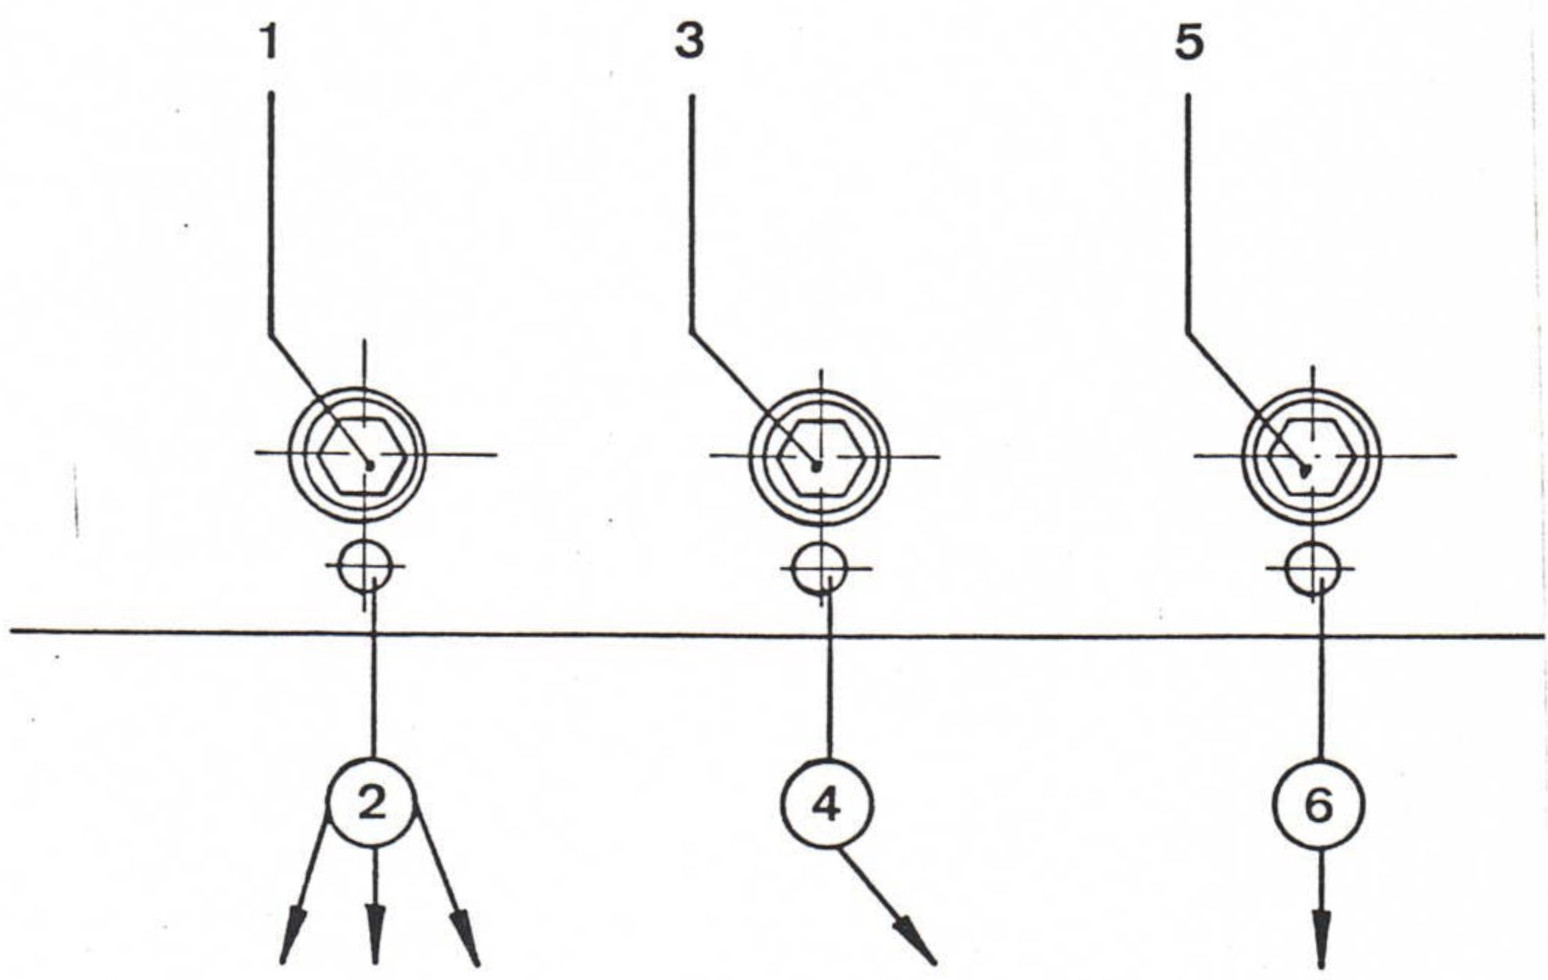
\includegraphics[width=0.8\textwidth]{manual_spindle_speed_selection.jpg}
    \label{fig:manual_spindle_speed_selection}
\end{figure}

\begin{table}[h]
    \centering
    \renewcommand{\arraystretch}{1.3}
    \begin{tabular}{|c|c|c|c|c|}
        \hline \hline
        \textbf{} & \textbf{Silver} & \textbf{Blue} & \textbf{Green} & \textbf{Color Combination} \\
        \hline \hline
        Speed   & 80    &   Spindle & 630  & Blue - Blue  \\
        (RPM)   & 100   &   Idle    & 800  & Blue - Red   \\
                & 125   &           & 1000 & Blue - Yellow \\
                &       &           &       &               \\
                & 160   &           & 1250 & Red - Blue  \\
                & 200   &           & 1600 & Red - Red   \\
                & 250   &           & 2000 & Red - Yellow \\
                &       &           &       &               \\
                & 315   &           & 2500 & Yellow - Blue \\
                & 400   &           & 3150 & Yellow - Red  \\
                & 500   &           & 4000 & Yellow - Yellow \\
        \hline \hline
    \end{tabular}
    \label{tab:spindle_speed}
\end{table}

\section{Horizontal Working Spindle}

\begin{figure}[h]
    \centering
    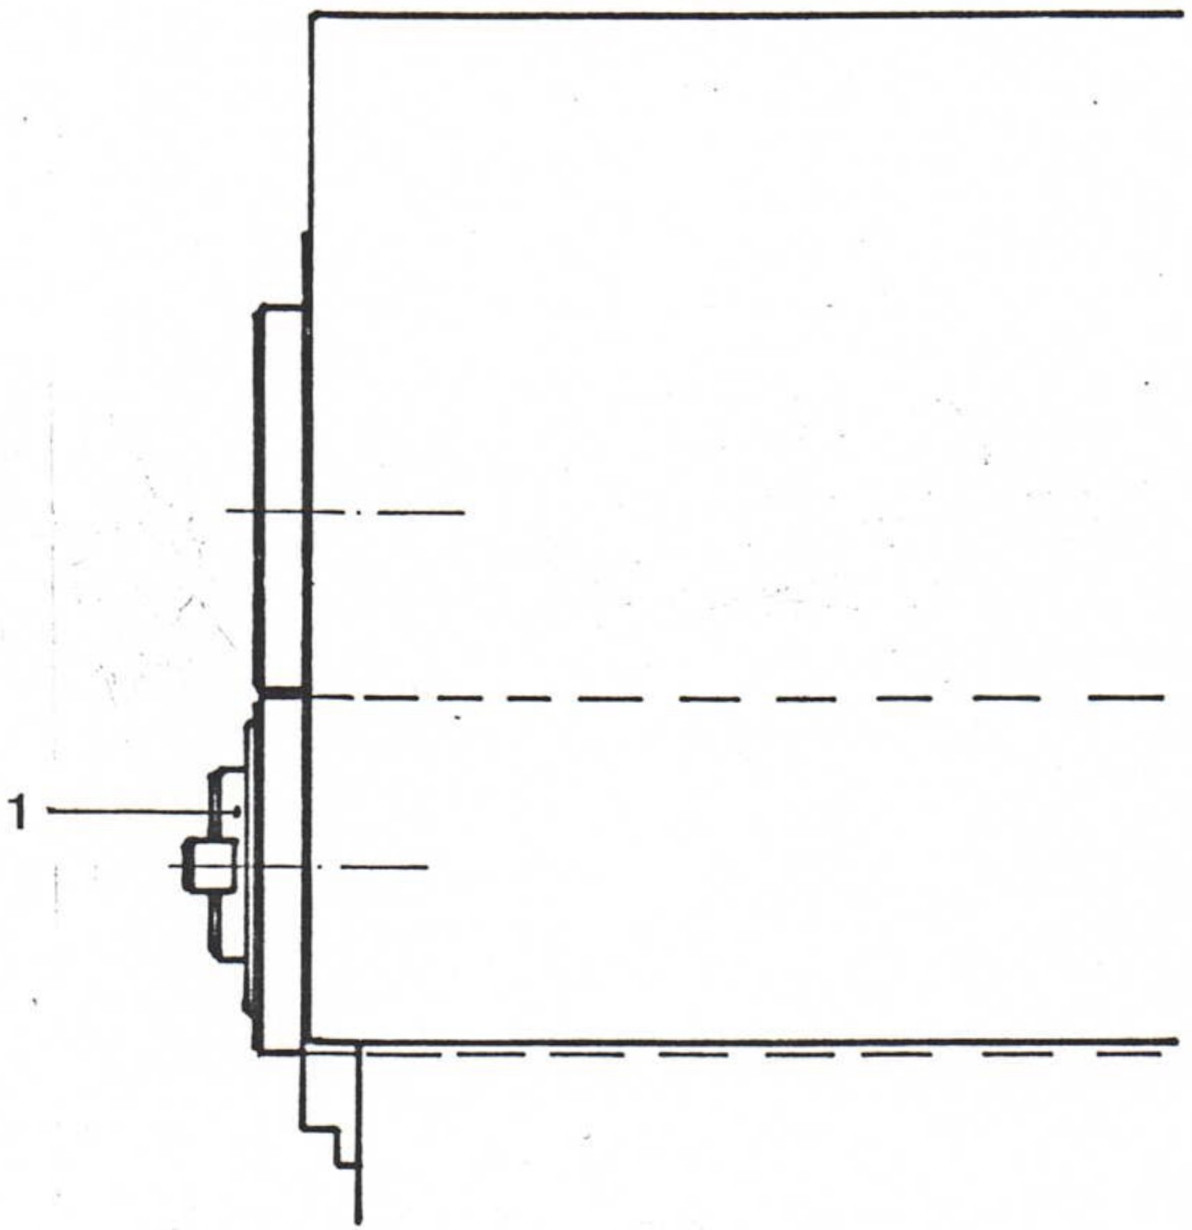
\includegraphics[width=0.7\textwidth]{horizontal_working_spindle.jpg}
    \label{fig:horizontal_working_spindle}
\end{figure}

\noindent \textbf{1} \quad Horizontal Working Spindle

\vspace{.5cm}

\notebox{NOTE}{The spindle bearings of the working spindle are \textbf{permanently lubricated} and therefore maintenance-free.}

\section{Horizontal Milling with Counter Holder}

\begin{figure}[h]
    \centering
    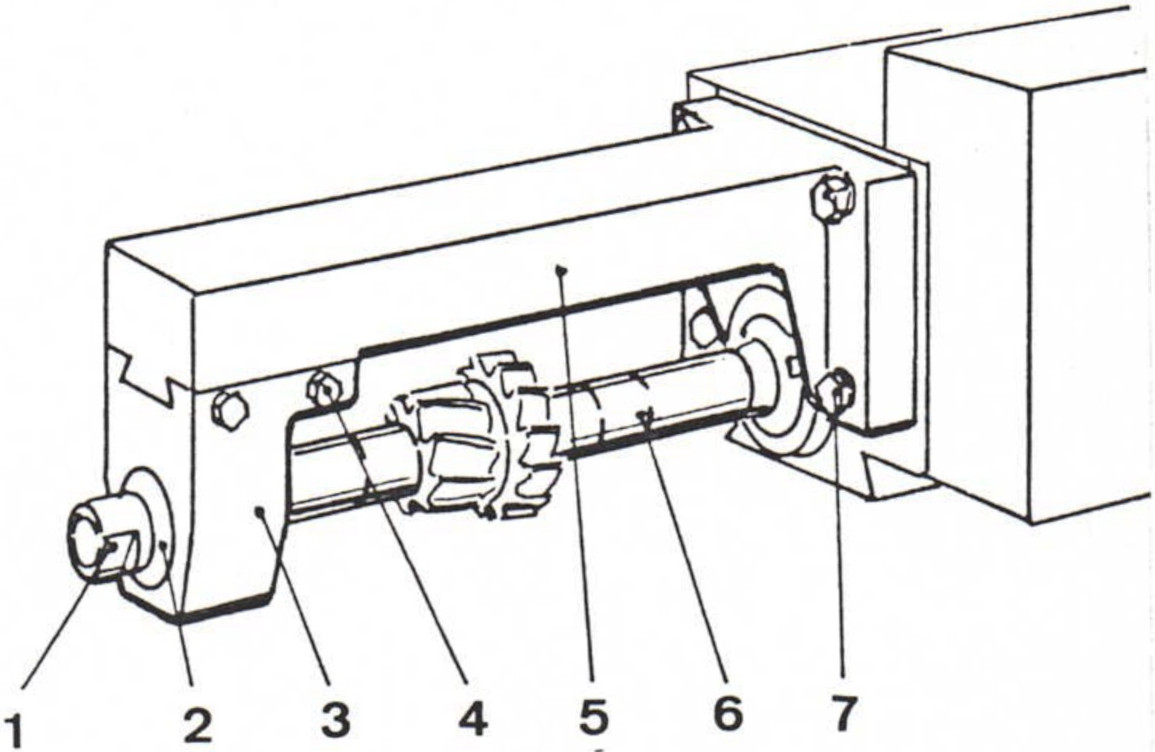
\includegraphics[width=0.8\textwidth]{horizontal_milling_counter_holder.jpg}
    \label{fig:horizontal_milling_counter_holder}
\end{figure}

\noindent \textbf{1} \quad Clamping Nut \\
\textbf{2} \quad Guide Bushing \\
\textbf{3} \quad Cutter Arbor Bearing \\
\textbf{4} \quad Screws \\
\textbf{5} \quad Counter Holder \\
\textbf{6} \quad Cutter Arbor \\
\textbf{7} \quad Hexagon Screws

\vspace{0.3cm}

\begin{itemize}
    \item Remove the tool from the vertical working spindle (see Sheet 3.12-1).
    \item Move the vertical milling head from the working position to the resting position (see Sheet 3.08-1).
    \item Attach the counter holder (5) to the spindle stock using hexagon screws (7).
    \item Insert the cutter arbor (6), equipped with milling cutters and rings, into the horizontal working spindle and tighten (see Sheet 3.12-1).
\end{itemize}

\notebox{NOTE}{Do not install the guide bushing (2) yet.}

\begin{itemize}
    \item Slide the cutter arbor bearing (3) into the dovetail guide of the counter holder (5).
    \item Insert the guide bushing (2) into the cutter arbor bearing (3) and slide it onto the cutter arbor (6).
    \item Screw on and tighten the clamping nut (1).
    \item Secure the cutter arbor bearing (3) using screws (4).
\end{itemize}

\noindent The removal of the counter holder follows the reverse sequence.\footnotemark

\vspace{0.3cm}

\footnotetext{The conversion from horizontal to vertical machining is described on Sheet 3.07-1.}

\section{Conversion from Horizontal to Vertical Machining}
\setcounter{section}{7}

\begin{figure}[h]
    \centering
    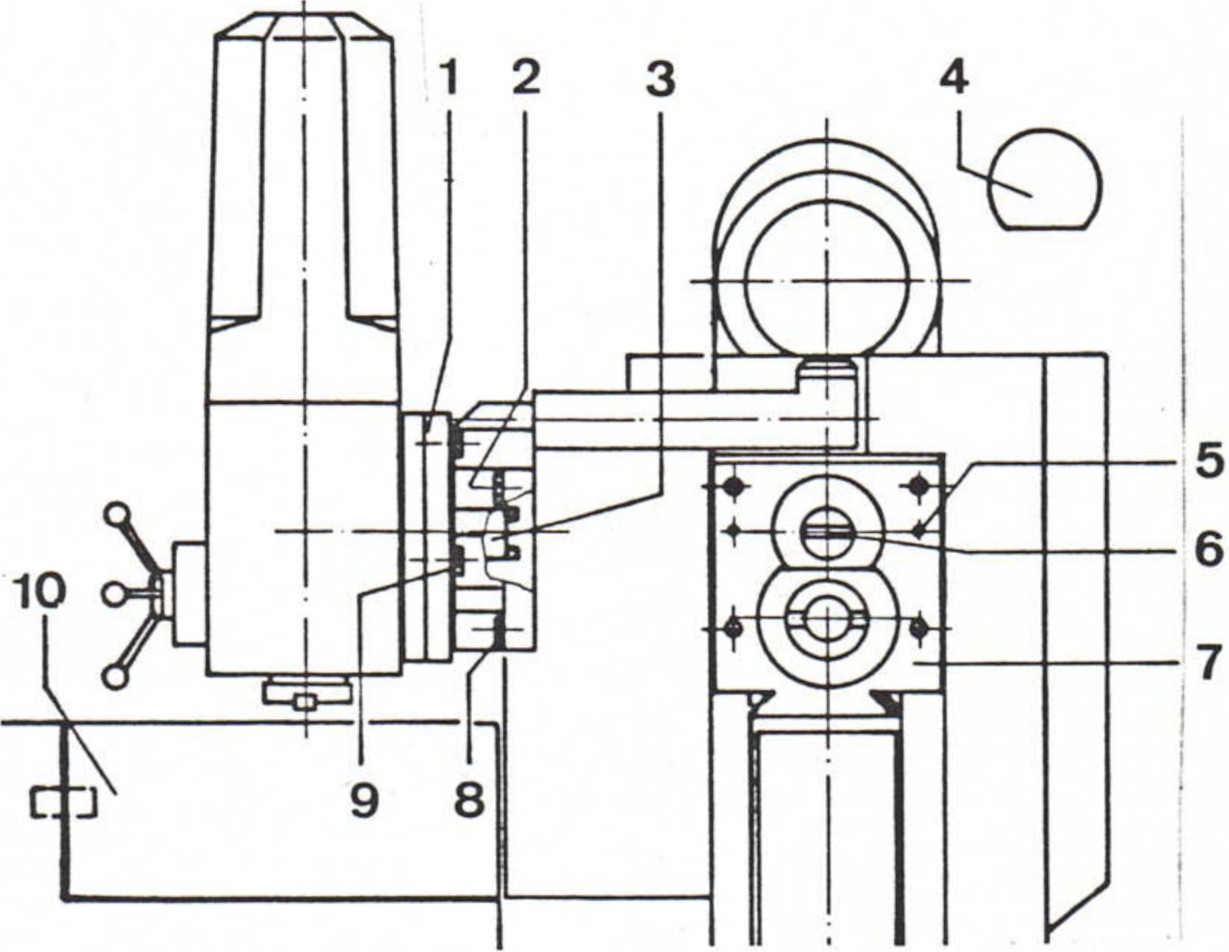
\includegraphics[width=0.8\textwidth]{horizontal_to_vertical_conversion.jpg}
    \label{fig:horizontal_to_vertical_conversion}
\end{figure}

\vspace{0.3cm}

\begin{itemize}
    \item Remove the tool from the horizontal working spindle (see Sheet 3.12-1).
    \item Move the table down to \enquote{+Y 370} and to the left to \enquote{-X 75}.\footnotemark
    \item Open the cover flap (10) in the splash guard back panel.
    \item Set the working spindle to idle mode (S0) (see Sheet 3.01-1).
    \item Remove the protective cover (4) from the coupling component (6).
    \item Rotate the coupling components (6) and (3) so that they engage properly, aligning the marks on the spindle stock (7) and intermediate flange (2).
    \item Release the vertical milling head lock and swing it from the rear rest position to the stop at the front of the spindle stock. Press on the centering pins (5) and secure it to the spindle stock using hexagon screws (8).
    \item Close the cover flap (10).
\end{itemize}

\vspace{0.3cm}

\subsection{Swiveling the Vertical Milling Head}

\begin{itemize}
    \item Loosen the hexagon screws (9) on the intermediate flange (2).
    \item Adjust the vertical milling head according to the scale (1) to the required angle.
    \item Tighten the hexagon screws (9).
\end{itemize}

\footnotetext{Coordinates and movement directions, see Sheet 2.03-1.}

\vspace{0.3cm}

\notebox{WARNING}{When the milling head is swiveled and the splash guard cabin is installed, the X-travel is restricted.}

\section{Conversion from Vertical to Horizontal Machining}

\begin{figure}[h]
    \centering
    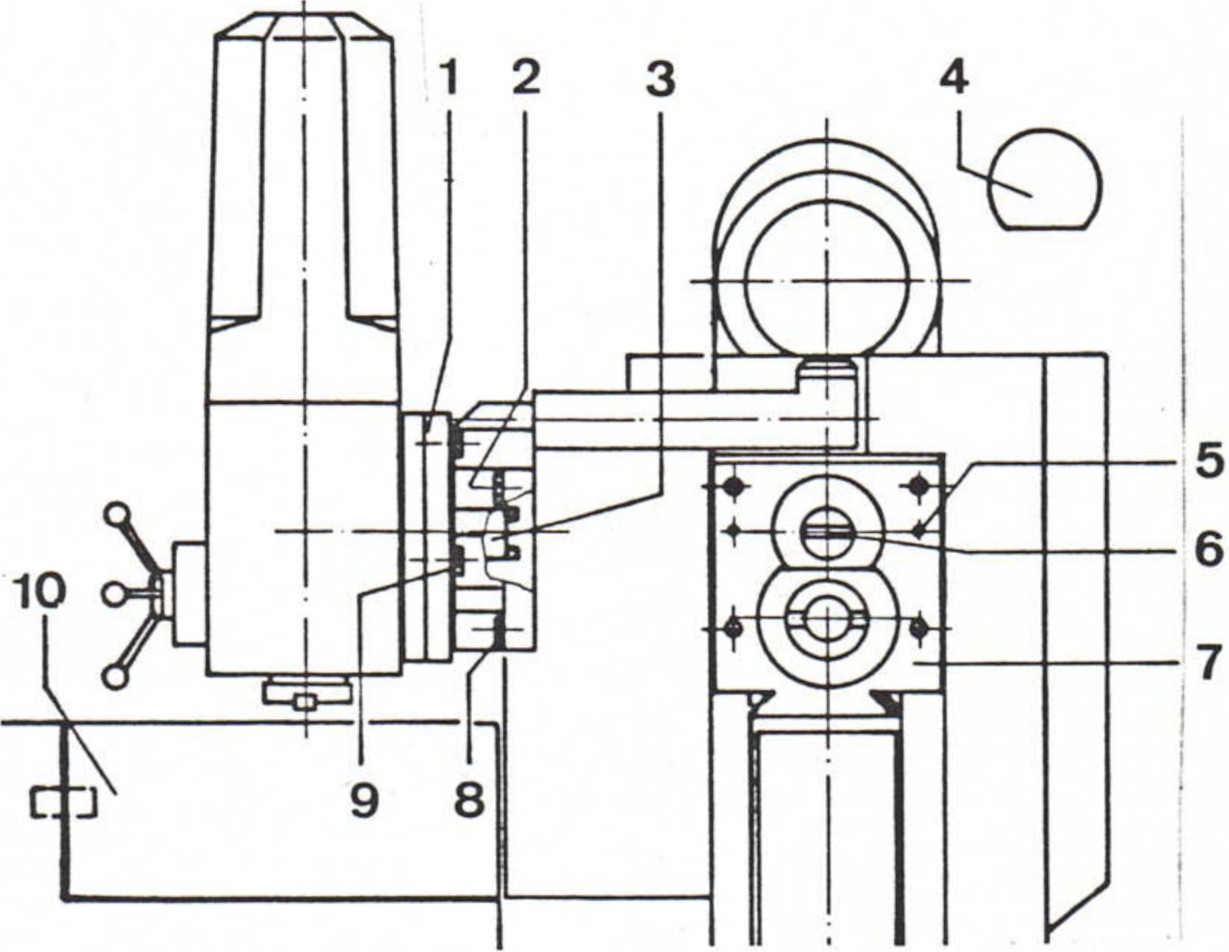
\includegraphics[width=0.8\textwidth]{horizontal_to_vertical_conversion.jpg}
    \label{fig:vertical_to_horizontal_conversion}
\end{figure}

\begin{itemize}
    \item Remove the tool from the vertical working spindle (see Sheet 3.12-1).
    \item Move the table down to \enquote{+Y 370} and to the left to \enquote{-X 75}.\footnotemark
    \item Open the cover flap (10) in the splash guard back panel.
    \item Remove the hexagon screws (8).
    \item Push the vertical milling head away from the spindle stock (7).
    \item Swing the vertical milling head sideways into its rear resting position and lock it.
    \item Close the cover flap (10).
\end{itemize}

\footnotetext{Coordinates and movement directions, see Sheet 2.03-1.}

\section{Vertical Milling Head Without PVG}

\begin{minipage}{0.5\textwidth}
    \begin{enumerate}[itemsep=1pt,parsep=0pt]
        \item Quill (maximum travel = 50 mm)
        \item Vertical working spindle
        \item Scale ring for reading quill adjustment (1 tick mark = 1 mm)
        \item Handwheel for adjusting the quill
        \item Locking screw for securing the quill
        \item Clamping screw for quill locking - Allen key: 6 mm SW
    \end{enumerate}
\end{minipage}%
\begin{minipage}{0.5\textwidth}
    \centering
    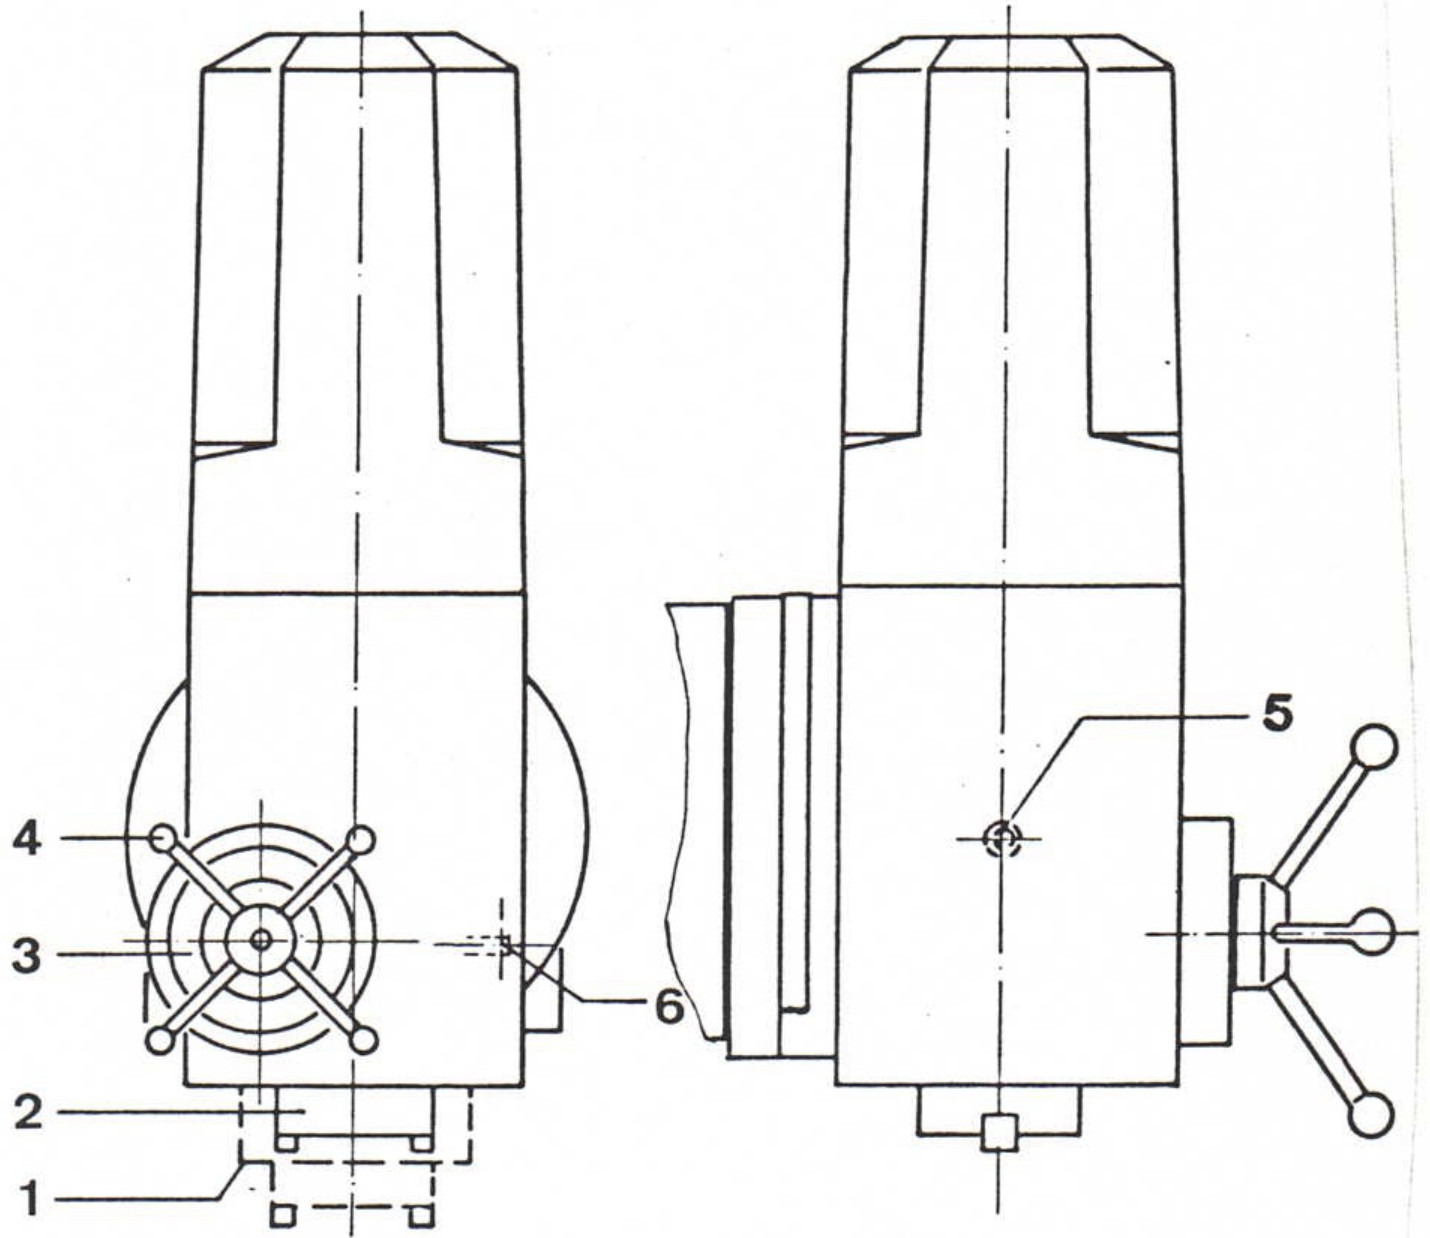
\includegraphics[width=0.9\textwidth]{vertical_milling_head_pvg.jpg}
\end{minipage}

\vspace{0.5cm}

\noindent The quill can be additionally secured beyond normal clamping.  
This is achieved using a\\ \textbf{toothed clamping block}, which engages with the \textbf{quill rack teeth} (1) when the locking screw (5) is turned clockwise.

\vspace{0.3cm}

\notebox{WARNING}{The quill locking mechanism allows secure positioning only within a range of \textbf{0-18.5 mm travel}, in increments of \textbf{3.125 mm}.}

\vspace{0.3cm}

\notebox{NOTE}{The spindle bearings feature \textbf{lifetime lubrication}, making them \textbf{maintenance-free}.}

\vspace{0.5cm}

\subsection{What is PVG?}

The term \textbf{PVG} in this context likely refers to a \textbf{quill positioning system}, such as a \textbf{fine-feed gearbox} or a \textbf{pneumatic-assisted movement}.

\begin{itemize}
    \item Some models may feature a \textbf{Precision Feed Gearbox (Präzisions-Vorschub-Getriebe)} for \\controlled quill movement.
    \item Others may include a \textbf{Pneumatic Adjustment System (Pneumatische Verstell-Garnitur)} to aid smooth positioning.
    \item Since this model is labeled \textbf{"without PVG"}, the quill must be \textbf{manually adjusted and locked} using screws.
\end{itemize}

\noindent In short, \textbf{machines with PVG provide finer control over quill movement}, whereas \textbf{this version requires manual force} to position and lock the quill.


\section{Automatic Tool Clamping}
\setcounter{section}{12}

The machine's two working spindles are equipped with an \textbf{automatic tool clamping} system.

\vspace{.3cm}

\noindent The tool is \textbf{permanently clamped} in the working spindle using \textbf{spring packs} and is released hydraulically.

\vspace{.3cm}

\noindent A \textbf{clamping collet} secures the tool in the working spindle by engaging a \textbf{groove ring} on the cylindrical part of the tool shank. This groove ring can be retrofitted onto\\ existing tools.\footnotemark

\footnotetext[1]{Reworking the shank of standard tools is explained on Sheet 3.13-1.}

\subsection{Clamping Force for Tool Clamping (ISO 40)}

\begin{itemize}[itemsep=1pt,parsep=0pt]
   \item MAHO/OTT Clamping Collet  \dotfill 11 kN \\
   \item ISO Type B Clamping Stud \dotfill \> 9.5 kN \\
  \item  Time for Clamping/Unclamping \dotfill \> approx. 3 s
\end{itemize}

\vspace{0.5cm}

\subsection{Tool Change} \footnotemark

\footnotetext[2]{Arrangement and function of CNC control elements on the command station are described in Section 10.7 of the CNC 432 Graphics manual.}

\begin{itemize}
    \item Stop the working spindle by pressing the \textbf{Spindle/Feed Stop} button on the CNC control panel.
    \item Press the \textbf{TOOL UNCL} button to release the tool.
    \item Remove the old tool from the working spindle.
    \item Insert the new tool into the working spindle and press the \textbf{TOOL UNCL} button again to clamp it.
\end{itemize}

\notebox{WARNING}{The tool must be fully inserted before clamping is completed; otherwise, the clamping collet may be damaged.}

\vspace{0.5cm}

\begin{minipage}{0.6\textwidth}
    \centering
    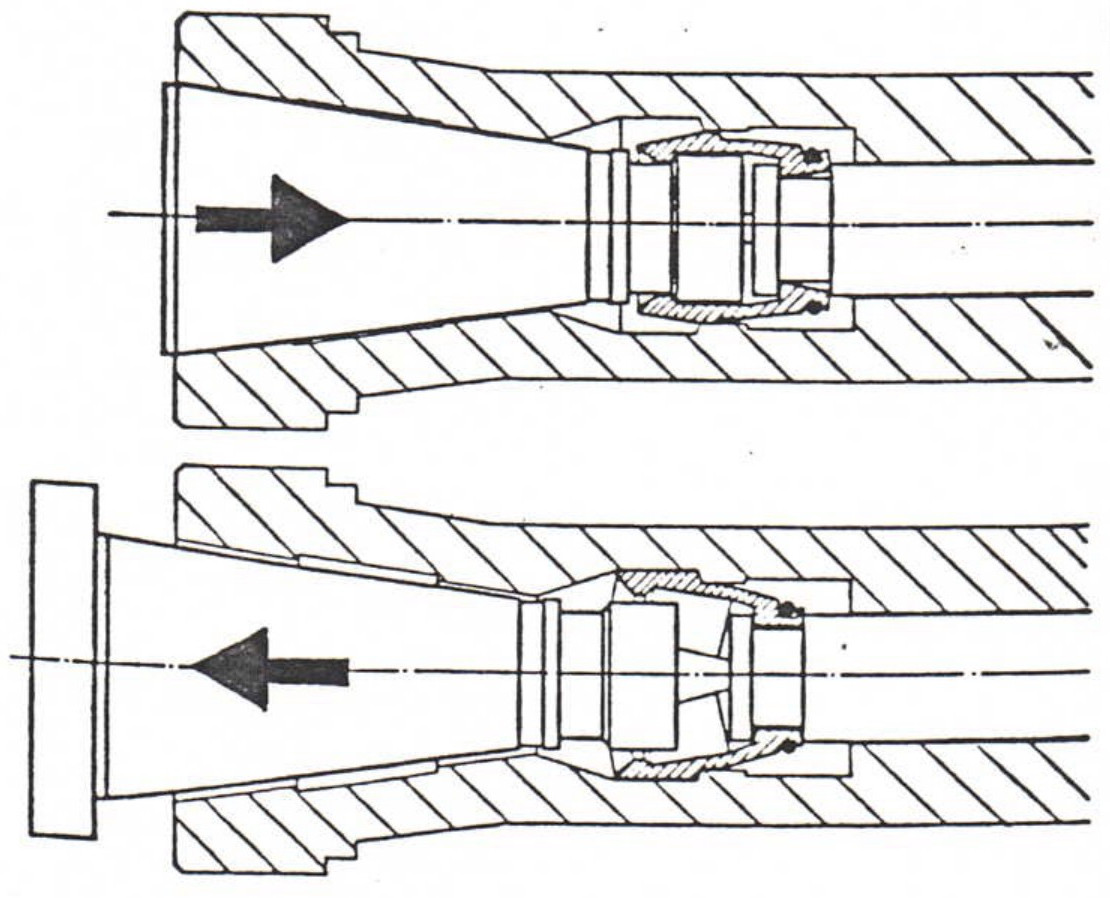
\includegraphics[width=0.9\textwidth]{tool_clamping.jpg}
\end{minipage}%
\begin{minipage}{0.4\textwidth}
   \textbf{Clamped Condition}
    \vspace{3.2cm}\\
   \textbf{Released Condition}
\end{minipage}

\section{Reworking the Shank of Standard Tools}

\textbf{MAHO/OTT, ISO 40}

\vspace{.5cm}

\noindent The ring groove on the shank of a standard tool must be modified.

\vspace{0.5cm}

\begin{minipage}{\textwidth}
    \centering
    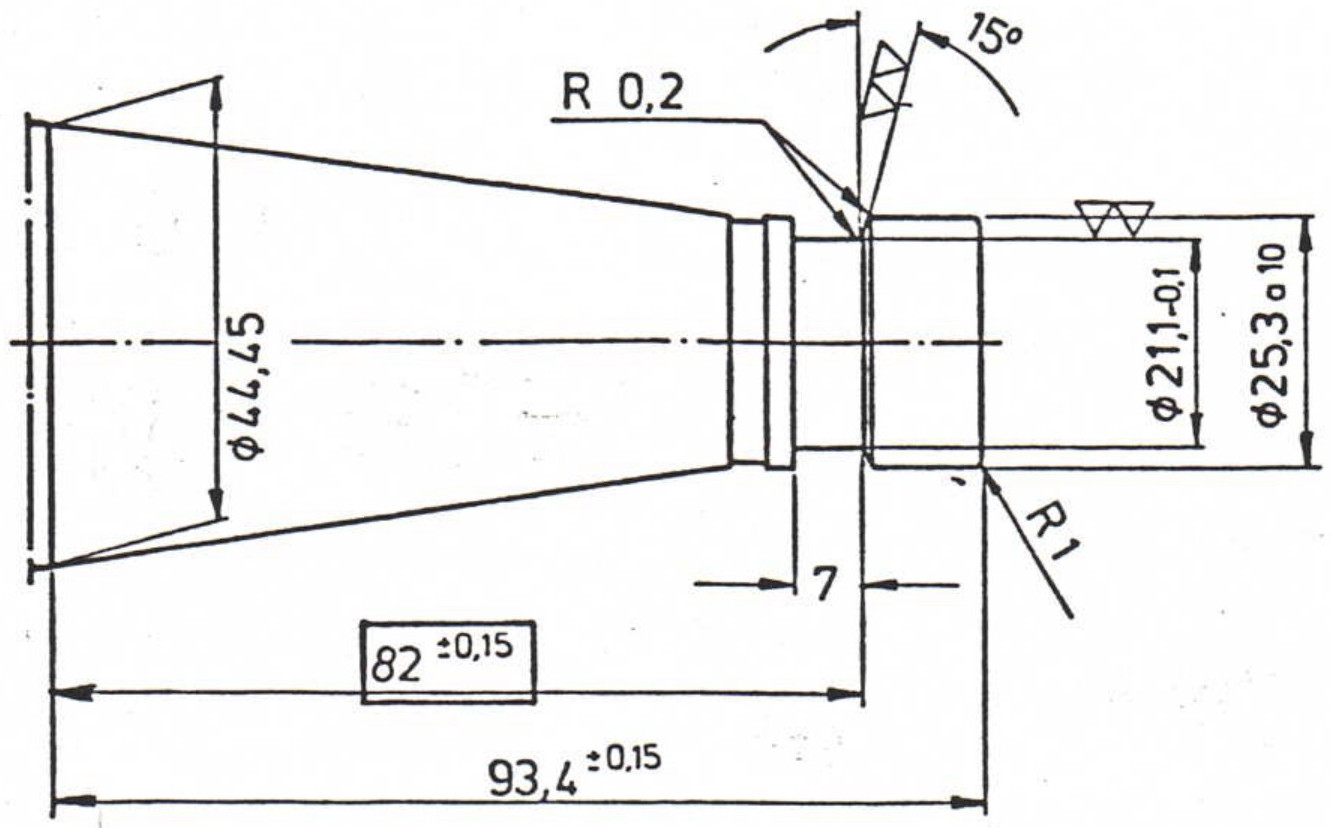
\includegraphics[width=0.8\textwidth]{tool_shank_rework.jpg}
\end{minipage}

\vspace{0.5cm}

\textbf{Checking the Ring Groove Using the MAHO Measuring Fixture}

\begin{enumerate}[itemsep=1pt,parsep=0pt]
    \item \textbf{Mounting Bushing}
    \item \textbf{Inspection Gauge}
\end{enumerate}

\vspace{0.5cm}

\begin{minipage}{\textwidth}
    \centering
    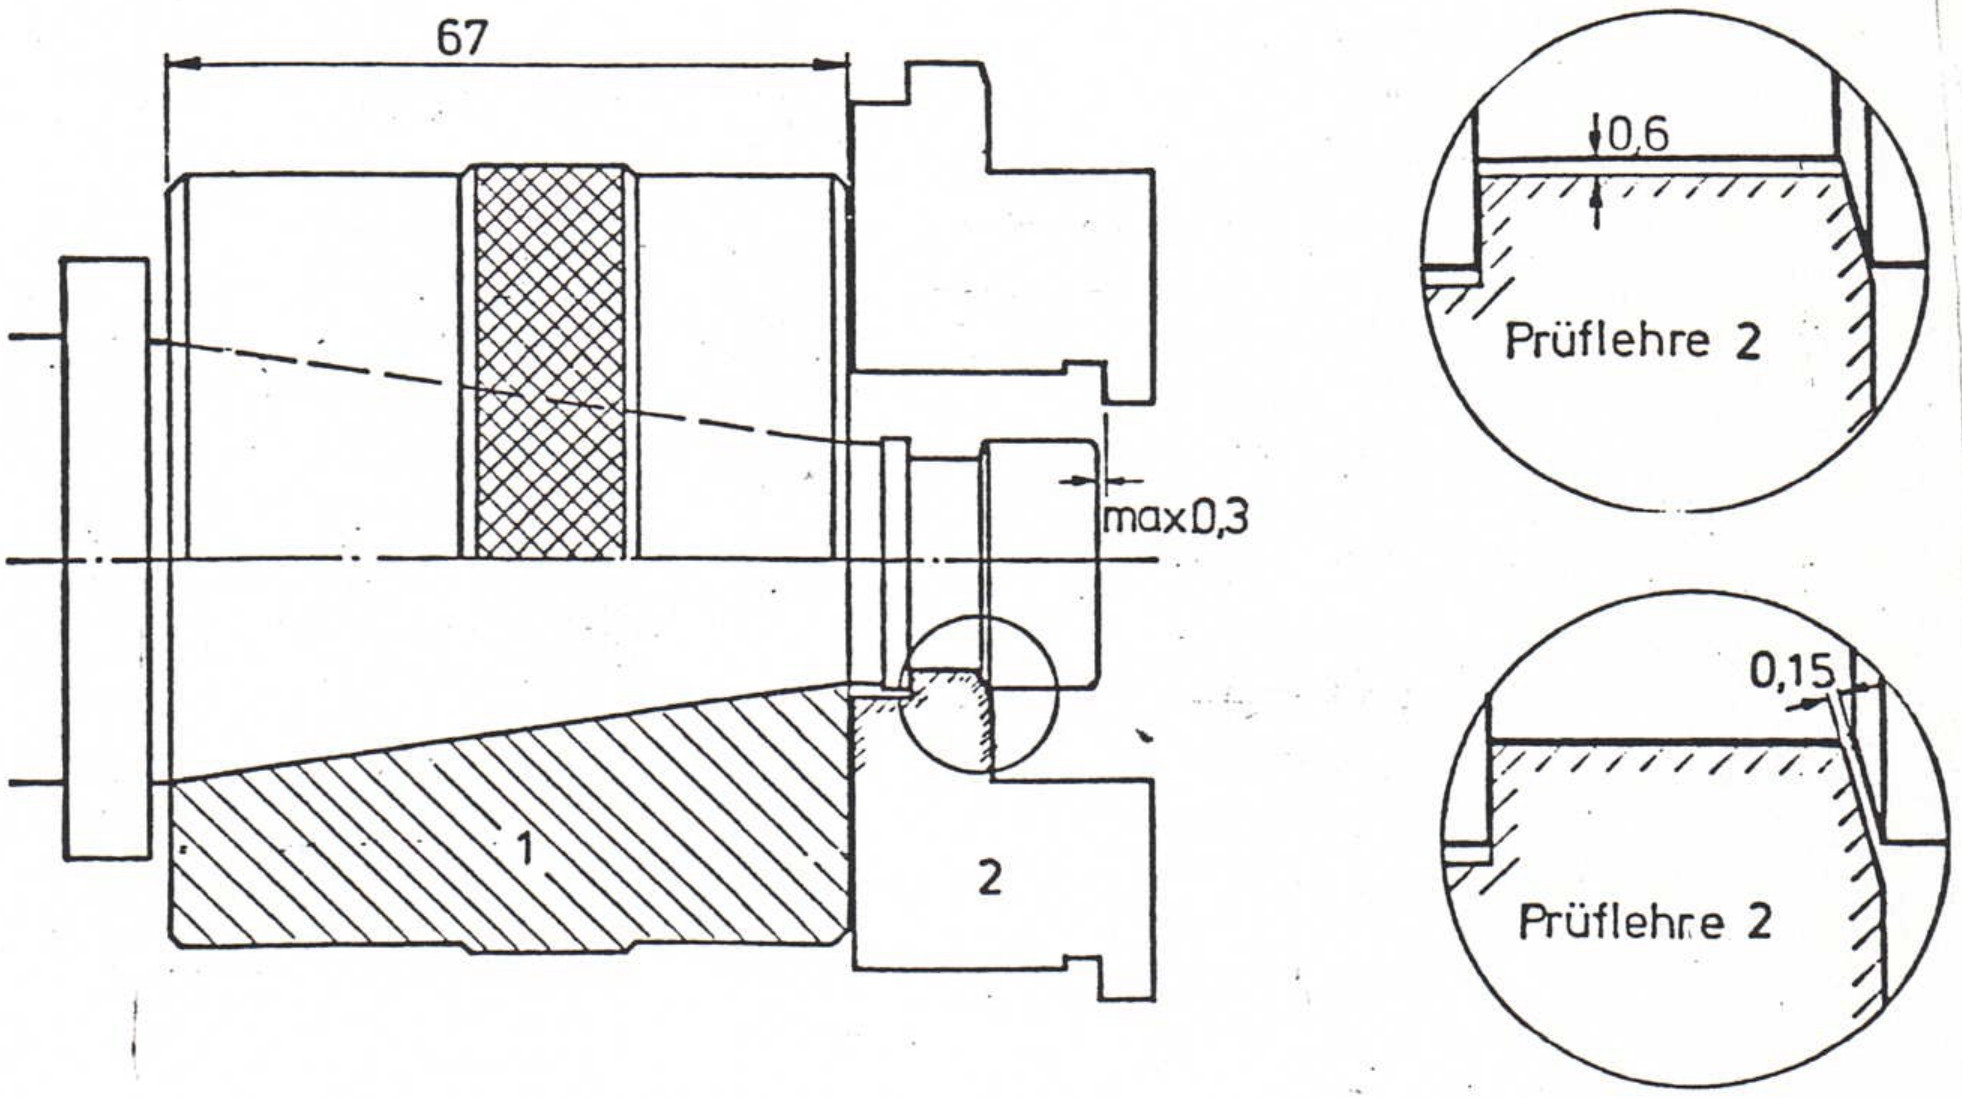
\includegraphics[width=0.8\textwidth]{ring_groove_inspection.jpg}
\end{minipage}

\vspace{0.5cm}

\noindent \textbf{See also Sheet 3.12-1.}

\sectionLikeSubsection{Tool Shank According to DIN 69871 with Pull Stud ISO 7388 Type B}

\setcounter{page}{3}

\textbf{ISO 40}

\vspace{0.5cm}

\begin{minipage}{\textwidth}
    \centering
    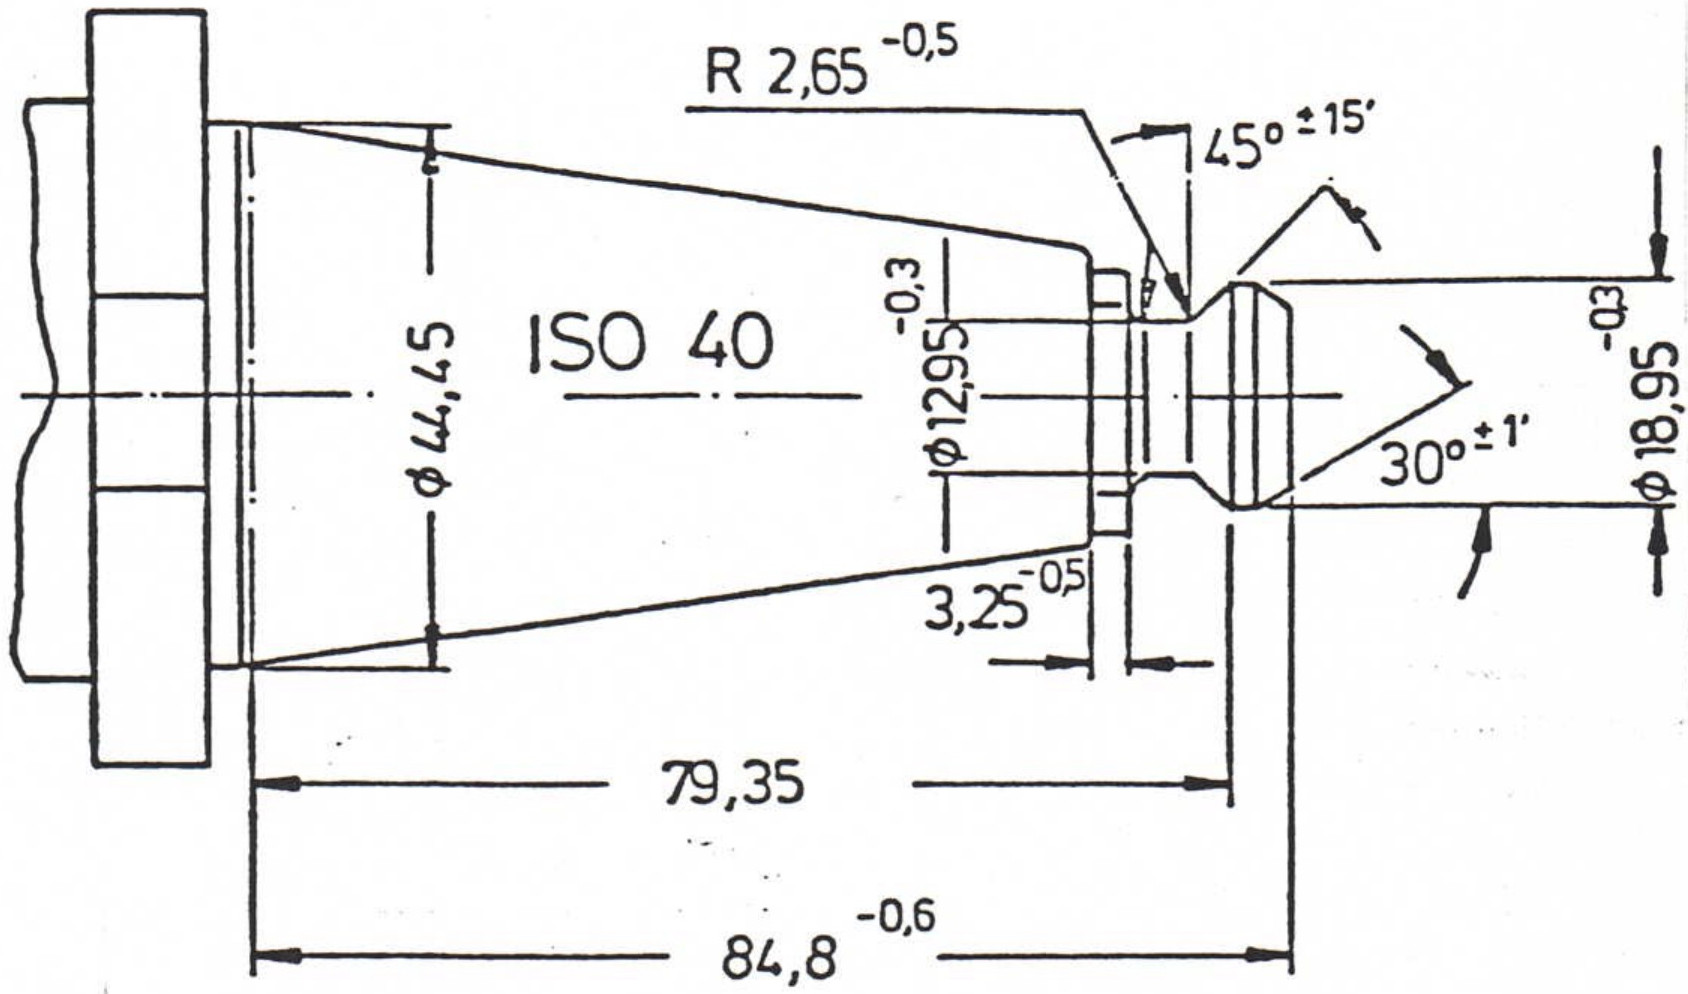
\includegraphics[width=0.8\textwidth]{tool_shank_iso40.jpg}
\end{minipage}

\vspace{0.5cm}

\textbf{Checking the Ring Groove Using the MAHO Measuring Fixture}

\begin{enumerate}[itemsep=1pt,parsep=0pt]
    \item \textbf{Mounting Bushing}
    \item \textbf{Inspection Gauge}
\end{enumerate}

\vspace{0.5cm}

\begin{minipage}{\textwidth}
    \centering
    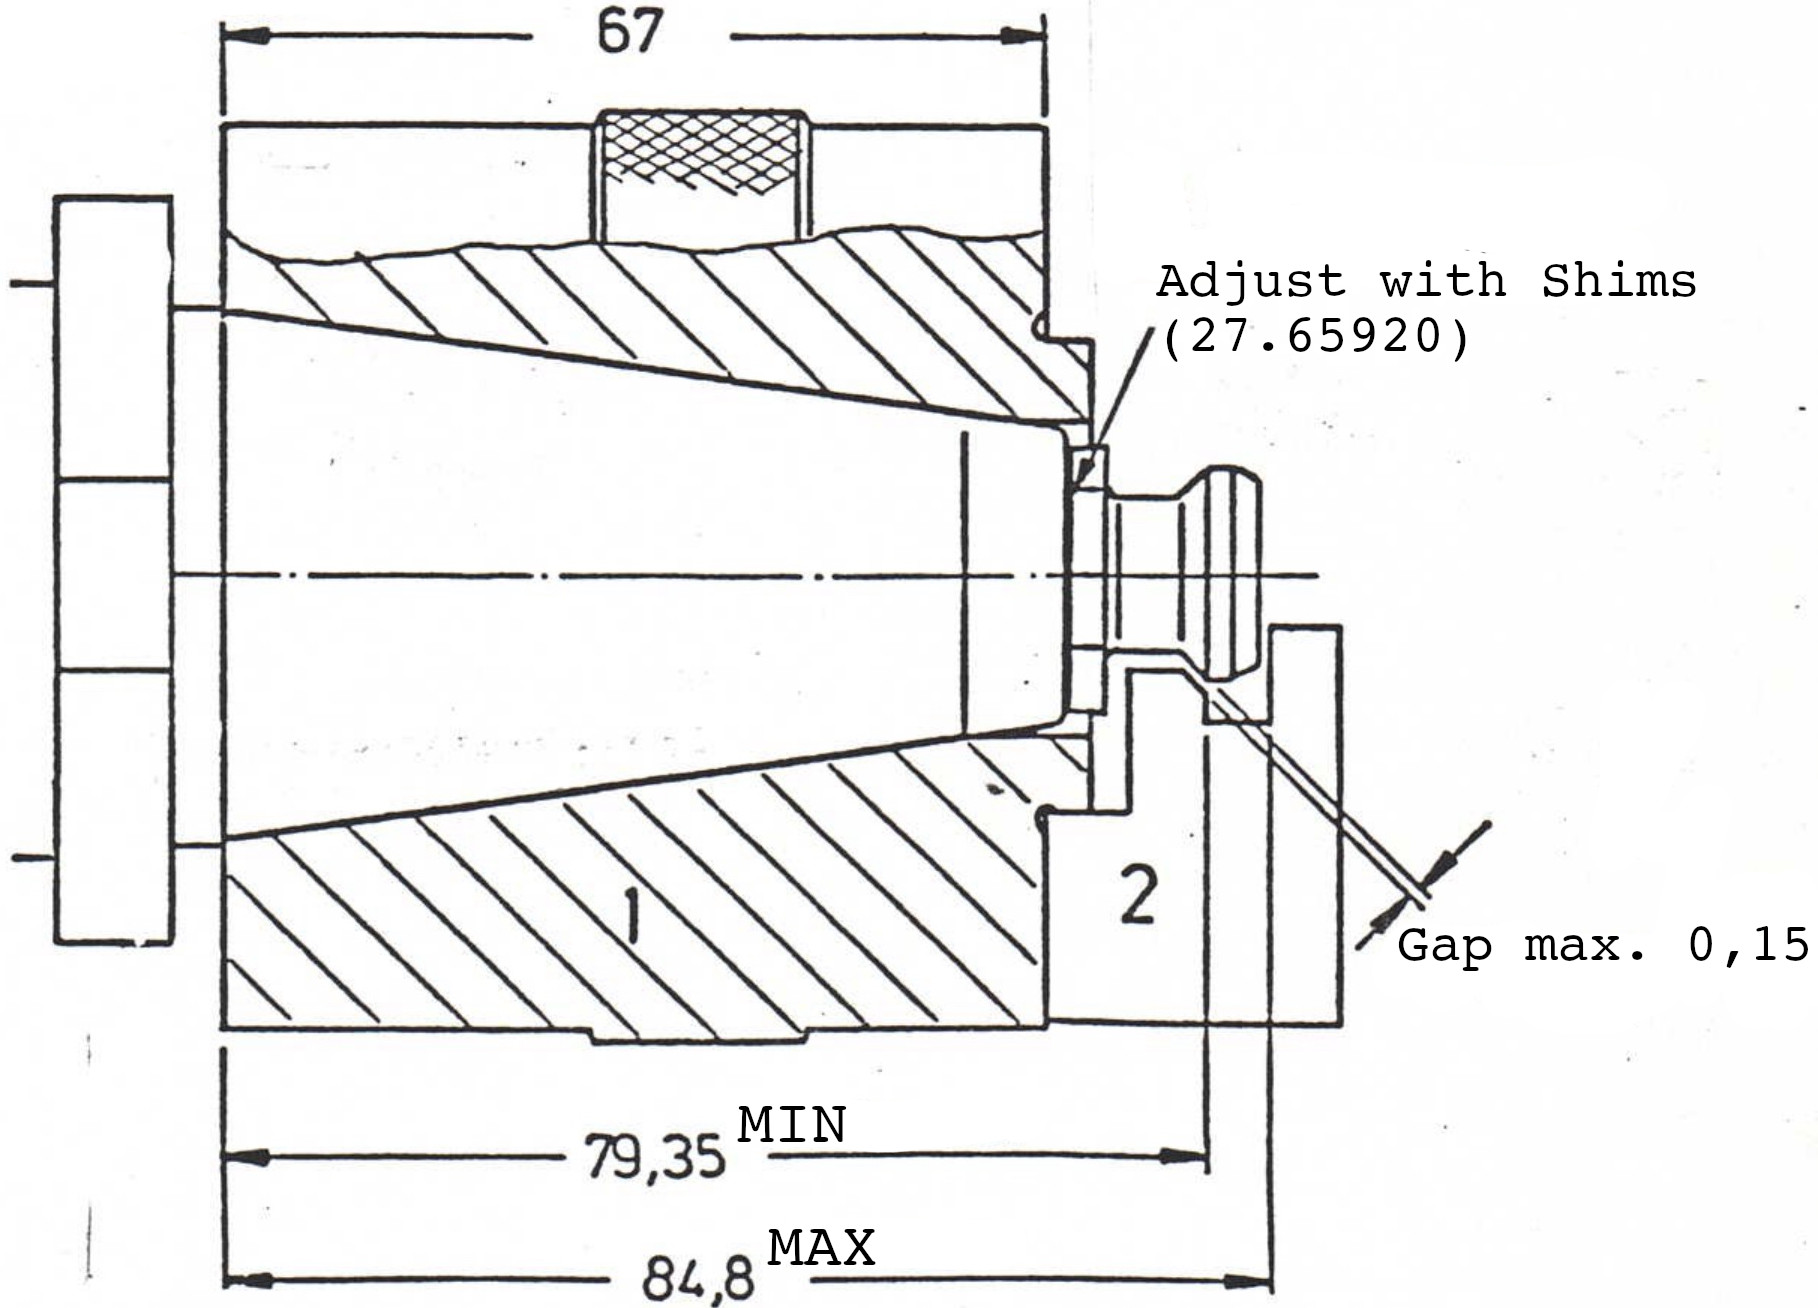
\includegraphics[width=0.7\textwidth]{ring_groove_measurement.jpg}
\end{minipage}

\vspace{0.5cm}

\noindent \textbf{See also Sheet 3.12-1.}

\section{Manually Resetting the Machine Carriage After an Emergency Stop}

\setcounter{page}{2}
\setcounter{section}{15}

If the normal travel range of the X, Y, or Z axes is exceeded due to a slip error, the machine is stopped by the \enquote{Emergency Stop} limit switch. The error \enquote{05} is displayed on the screen.

\vspace{.3cm}

\noindent To restart the machine, the carriages must be manually moved back. This is done by rotating the motor shafts approximately 3-5 turns until the emergency stop limit switch is released.

\vspace{.3cm}

\noindent Afterward, clear error \enquote{05} and reapproach the reference point.

\vspace{.3cm}

\notebox{WARNING}{%
Before resetting the Y-axis, open the control cabinet, hold the motor shaft using a double-ended wrench (5), then set the rotary switch \enquote{Y-Axis Brake} (on the adjustment module) to \enquote{Release}. After moving out of the emergency stop area, return the switch to \enquote{Brake Engaged}.
}

\notebox{NOTE}{%
For \enquote{Clearing Error Messages}, see the CNC control manual.
}

\noindent \textbf{Required tools from the standard accessories:}\\
(1) Hex screwdriver, (3) Square socket wrench, (5) Double-ended wrench

\vspace{2cm}

\noindent \textbf{The motor shafts are accessible at the following locations:}  

\begin{textblock*}{\textwidth}(10.5cm, 11.5cm)
\begin{itemize}
    \item \textbf{X-Axis:} After removing the cap (2).  
    \item \textbf{Y-Axis:} After removing the sheet metal cover (4) \\- under the control cabinet.  
    \item \textbf{Z-Axis:} Through the borehole in the top cover.  
\end{itemize}

\vspace{0.3cm}

\notebox{NOTE}{%
Counterclockwise rotation results in \\movement as follows:
\begin{itemize}
    \item \textbf{-X}: Table moves left.
    \item \textbf{-Y}: Support moves upwards.
    \item \textbf{-Z}: Spindle stock moves backward.
\end{itemize}
}

\end{textblock*}

\begin{minipage}{\textwidth}
    \centering
    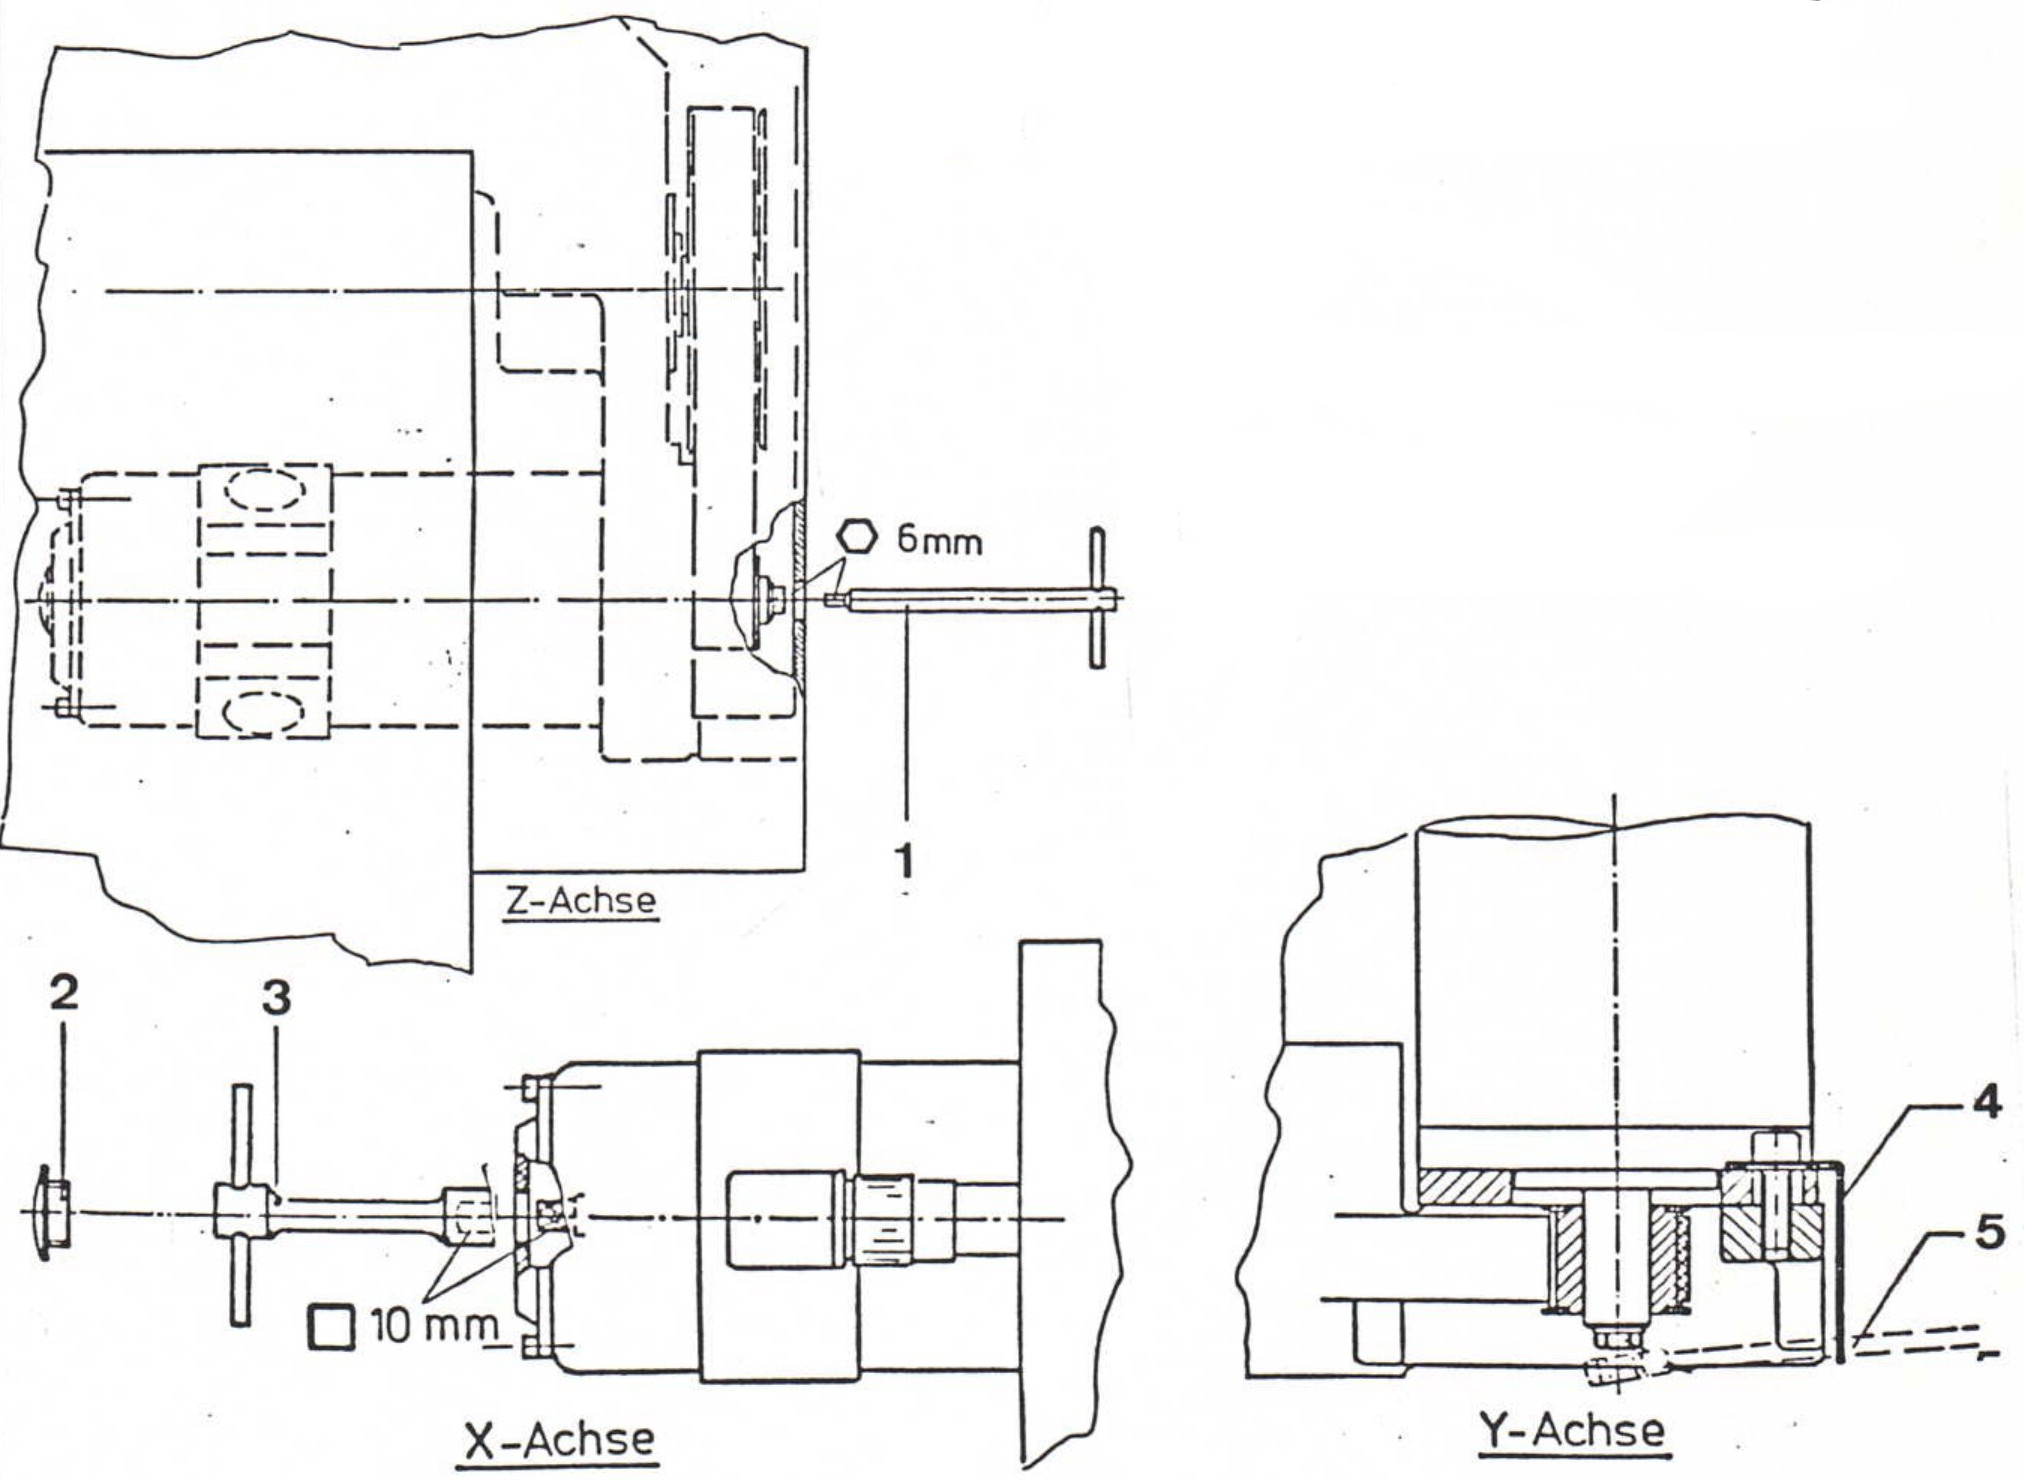
\includegraphics[width=0.9\textwidth]{machine_carriage_reset.jpg}
\end{minipage}

\section{Hydraulic Diagram}
\setcounter{section}{18}

\begin{figure}[h]
    \centering
    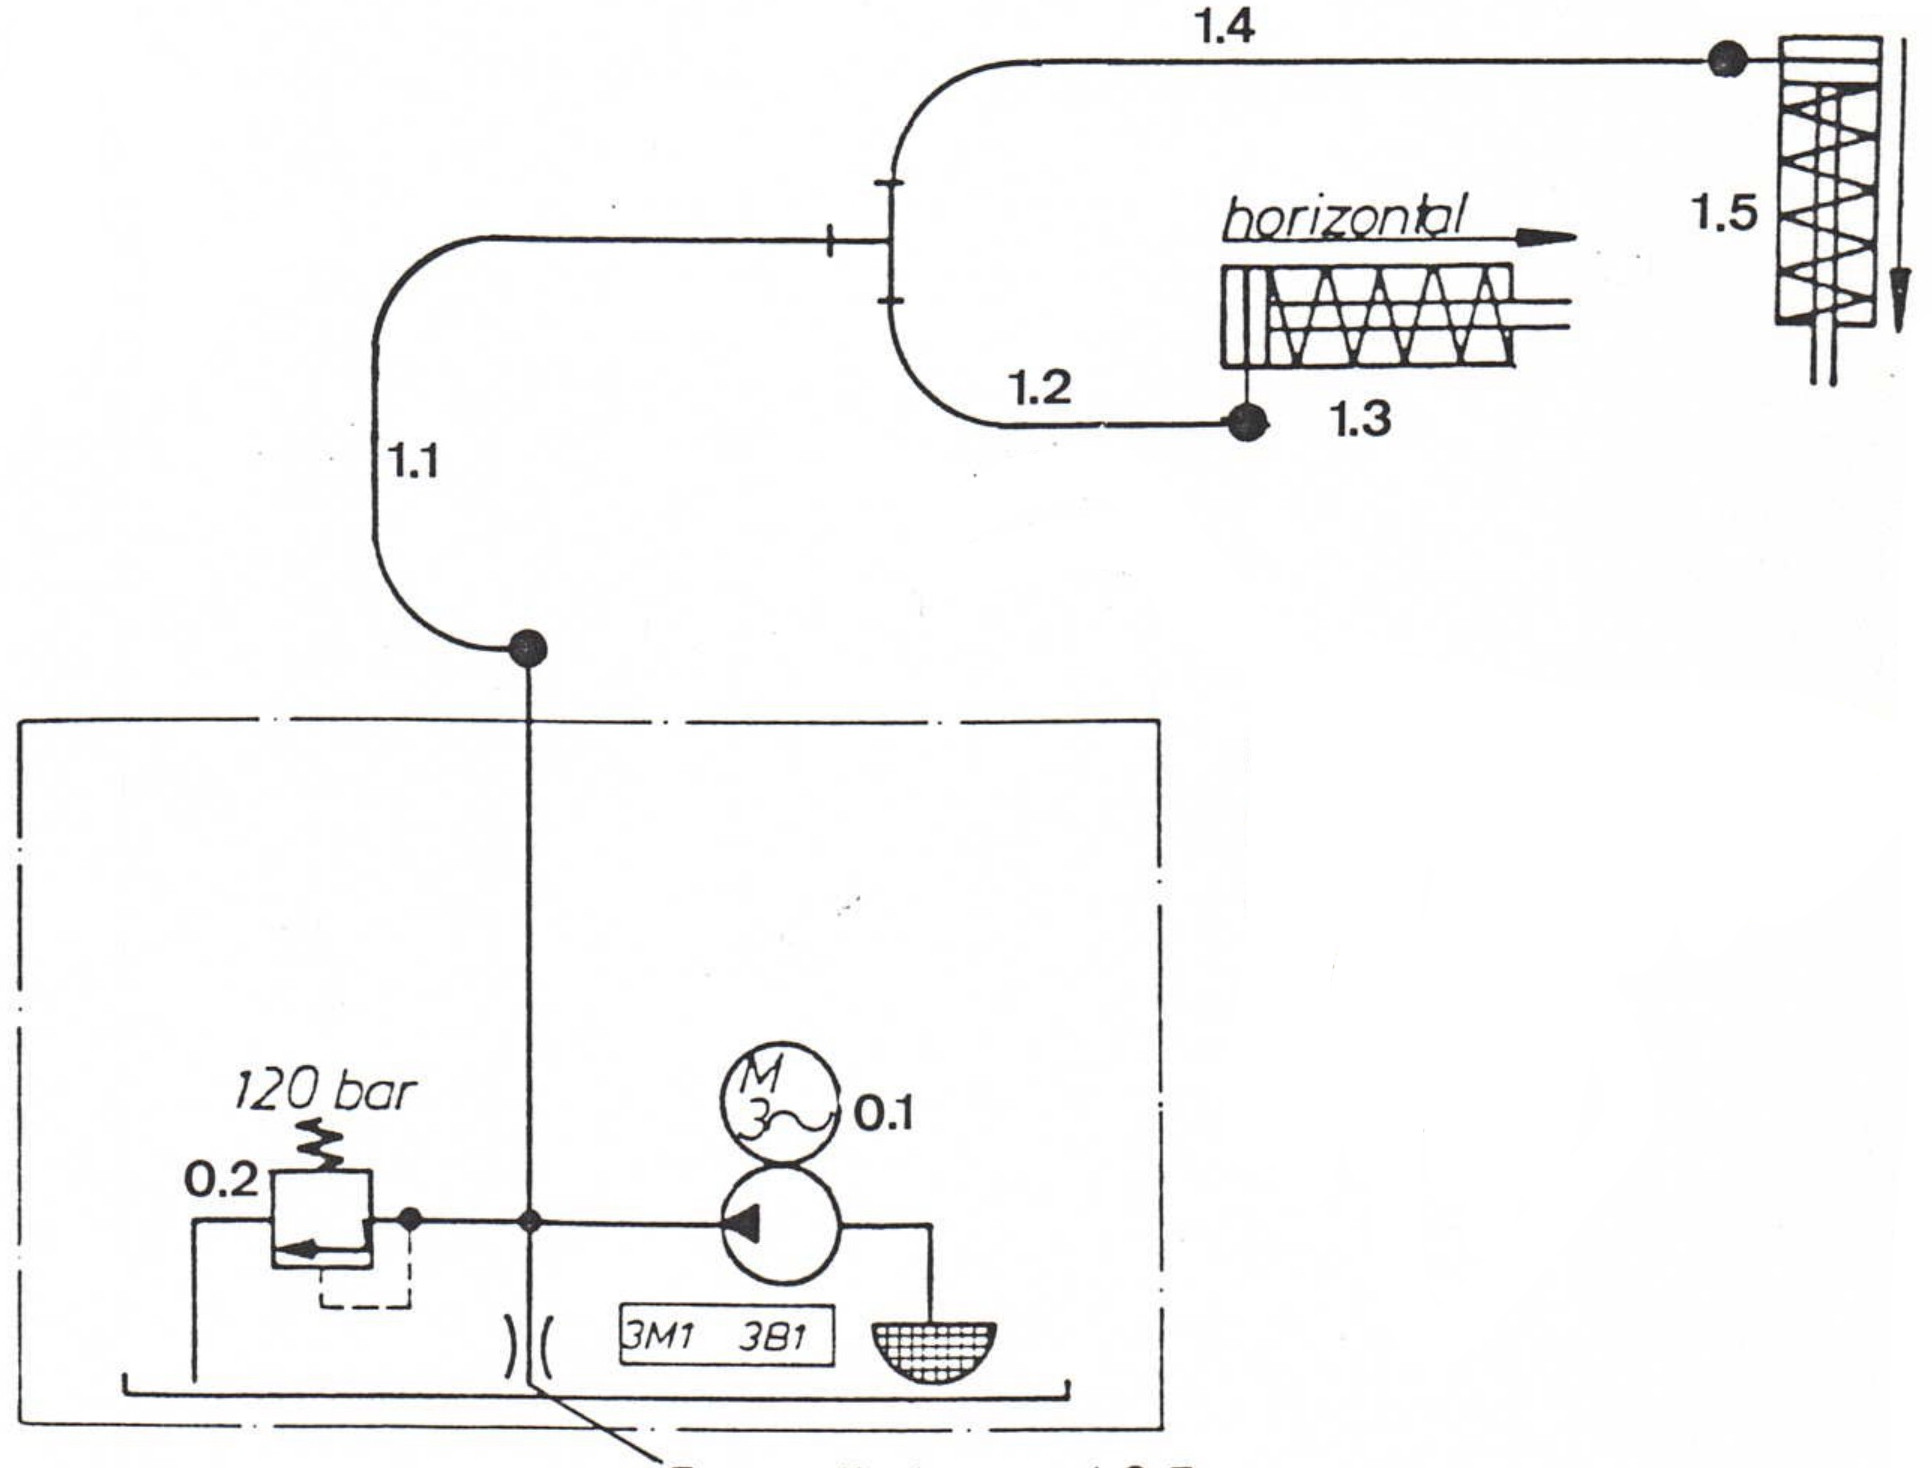
\includegraphics[width=.95\textwidth]{hydraulic_diagram.jpg}
\end{figure}

\begin{textblock*}{\textwidth}(12.7cm, 9.3cm)
    \noindent
    \textbf{Oil Volume:} Total 2.01 l, Usable 1.3 l \\
    \textbf{Oil Type:} CL 46 DIN 51502 \\
    \textbf{Flow Rate:} $Q = 1.81 \text{ l/min}$ \\
    \textbf{Power:} $P = 0.37 \text{ kW}$ \\
    \textbf{Pump Speed:} $n = 2810 \text{ min}^{-1}$
\end{textblock*}

\begin{textblock*}{\textwidth}(7cm, 15.5cm)
    \textbf{throttle bore} \O0,5
\end{textblock*}

\subsection{Hydraulic Equipment List}

\begin{table}[h]
    \centering
    \begin{tabularx}{\textwidth}{|l|l|l|l|l|}
        \hline
        \textbf{Plan}   & \textbf{Ident-Nr.}    & \textbf{Description}      & \textbf{Specification}    & \textbf{Manufacturer} \\
        \textbf{Nr.}    &                       &                           &                           &                       \\
        \hline
        \hline
        0.1             & 27.70463              & Hydraulic compact unit     & N. Stückl.               & HAWE                  \\
                        &                       & SK 7611                    & 7310 700                 &                       \\
        0.2             & (in Pos.              & Pressure limiting valve    &                          & HAWE                  \\
                        & 0.1)                  &                            &                          &                       \\
        1.1             & 81.22225              & Hydraulic line             & AF4 2300 mm              & Tecalemit             \\
        1.2             & 81.22221              & Hydraulic line             & AF4 2300 mm              & Tecalemit             \\
        1.3             & 27.67898              & Clamping head, horizontal  & 95.100.366.3.2           & Ott                   \\
        1.4             & 81.15108              & Hydraulic line             & AF4 1700 mm              & Tecalemit             \\
        1.5             & 27.69738              & Clamping head, vertical    & 95.100.558.2.2           & Ott                   \\
        \hline
    \end{tabularx}
    \label{tab:hydraulic_list}
\end{table}

\sectionLikeSubsection{Hydraulic System}
\setcounter{page}{3}

\begin{figure}[h]
    \centering
    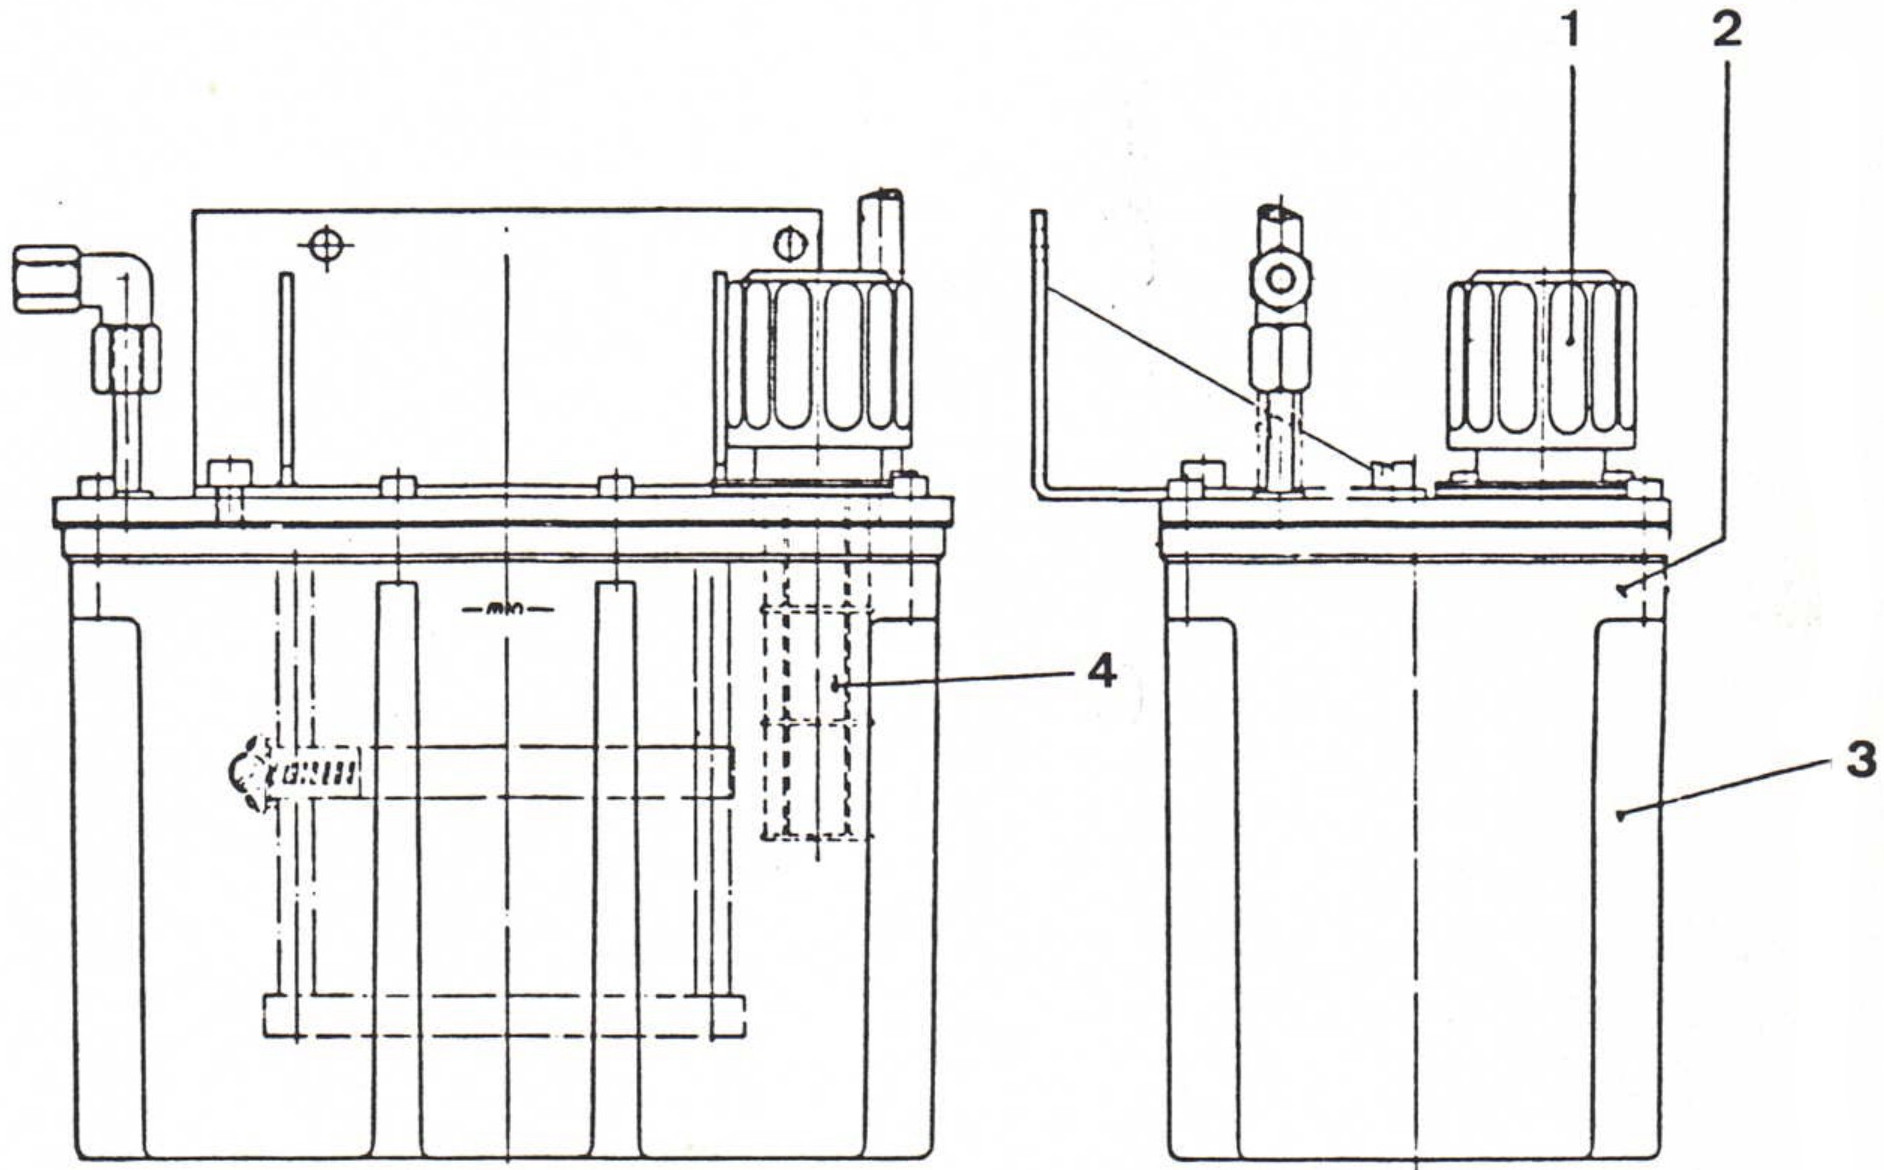
\includegraphics[width=0.8\textwidth]{hydraulic_unit.jpg}
    \label{fig:maho_hydraulic_unit}
\end{figure}

\begin{enumerate}
    \item \textbf{Filler Neck} \footnotemark
    \item \textbf{Hydraulic Unit}
    \item \textbf{Transparent Container}
    \item \textbf{Oil Strainer}
\end{enumerate}

\footnotetext[1]{See Sheet \textbf{7.06-1}, \textit{"Lubrication Recommendations"}.}

\notebox{warning}{When refilling oil, ensure maximum cleanliness.  
The oil strainer must be thoroughly cleaned.}

\subsection{Functionality}  \footnotemark
\footnotetext[2]{Layout and function of the control station elements, see Sheet \textbf{2.04-1}.}

\textit{(See hydraulic diagram, Sheet 3.18-1)}

\noindent Pressing the illuminated push button \textbf{-3SH1-} on the control station starts the  
pump of the hydraulic unit and, within a few seconds, builds up the operating  
pressure of approximately \textbf{115 bar} required for releasing the tool clamps.  

\vspace{0.3cm}

\noindent The indicator light \textbf{-3H1-} on the control station illuminates, indicating  
that the operating pressure of the hydraulic system is present.

\section{Automatic Central Lubrication System}

\setcounter{section}{20}

\begin{figure}[h]
    \centering
    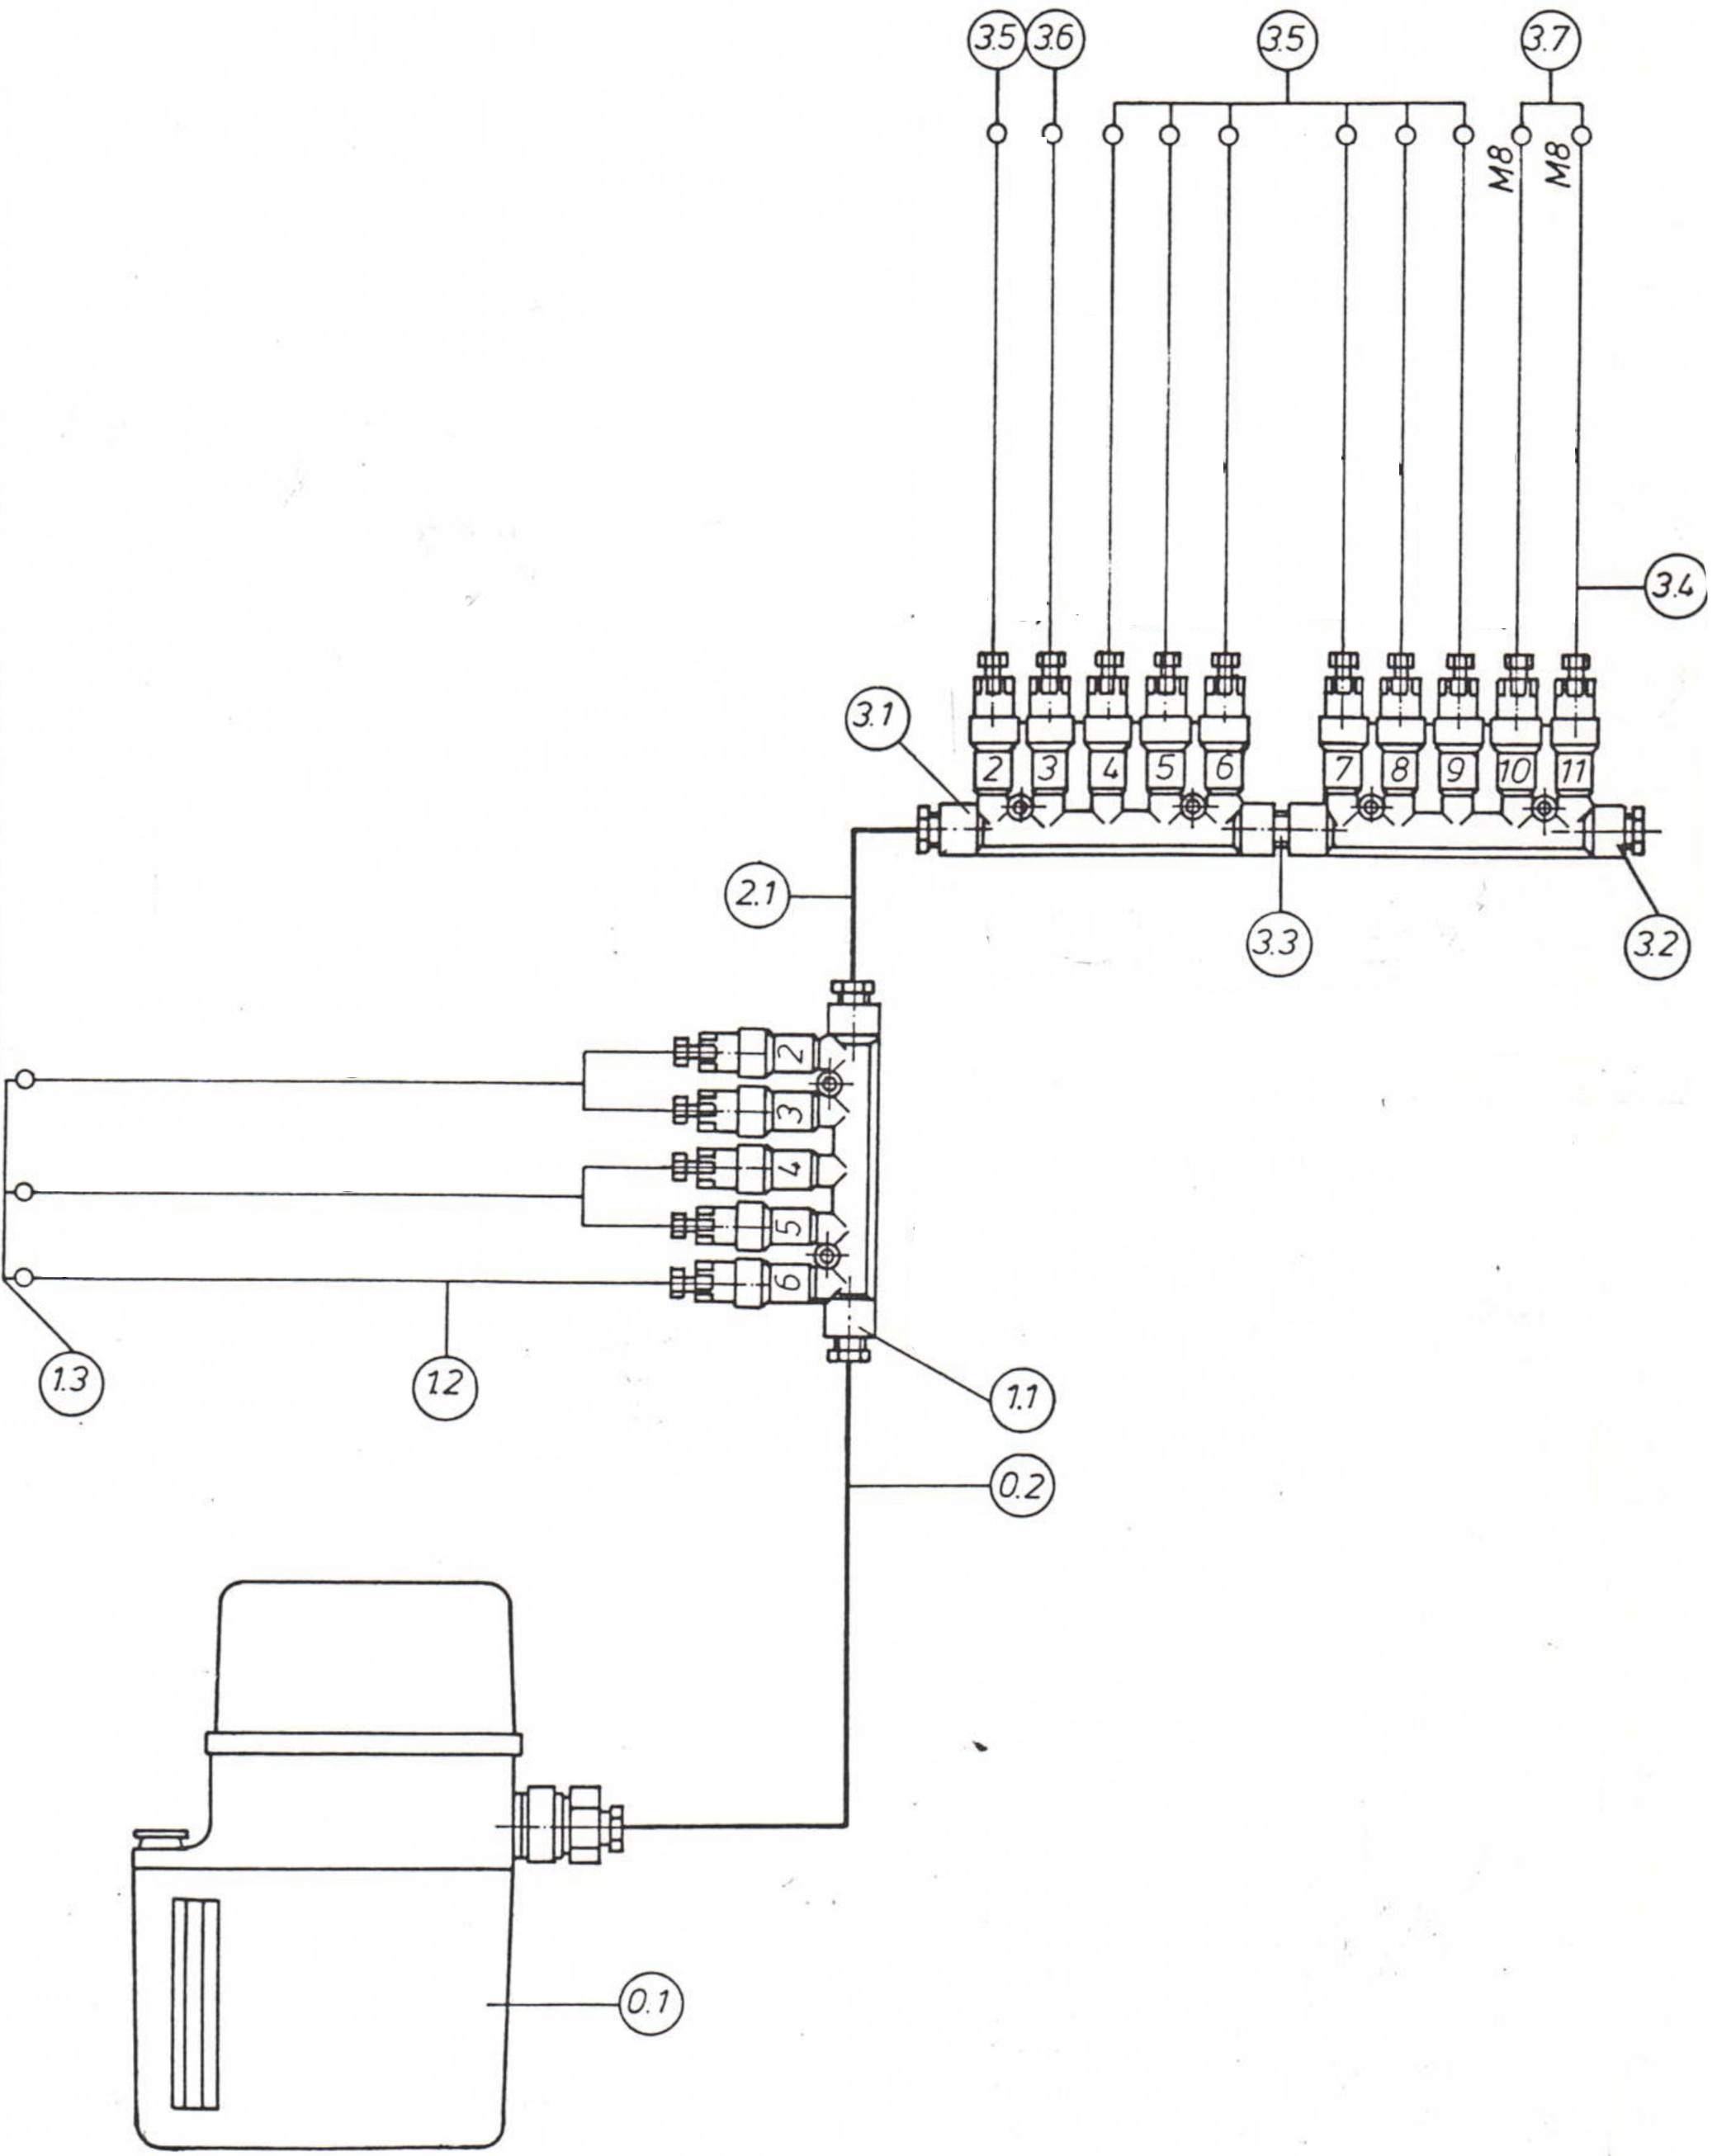
\includegraphics[width=0.8\textwidth]{central_lubrication.jpg}
    \label{fig:maho_central_lubrication}
\end{figure}

% Bottom-aligned rotated labels
\begin{textblock*}{3cm}(10.8cm,4.8cm)
    {\rotatebox{90}{\textbf{Spindle Nut X-Axis}}}
\end{textblock*}

\begin{textblock*}{3cm}(11.3cm,3.85cm)
    {\rotatebox{90}{\textbf{Spindle Nut Y-Axis M8x1}}}
\end{textblock*}

\begin{textblock*}{3cm}(11.75cm,4.95cm)
    {\rotatebox{90}{\textbf{X-Surface, Bottom}}}
\end{textblock*}

\begin{textblock*}{3cm}(12.2cm,5.4cm)
    {\rotatebox{90}{\textbf{Y-Surface, Left}}}
\end{textblock*}

\begin{textblock*}{3cm}(12.65cm,5.2cm)
    {\rotatebox{90}{\textbf{Y-Guidance, Left}}}
\end{textblock*}

\begin{textblock*}{3cm}(13.55cm,5.15cm)
    {\rotatebox{90}{\textbf{Y-Surface, Right}}}
\end{textblock*}

\begin{textblock*}{3cm}(14cm,5cm)
    {\rotatebox{90}{\textbf{Y-Guidance, Right}}}
\end{textblock*}

\begin{textblock*}{3cm}(14.45cm,5.15cm)
    {\rotatebox{90}{\textbf{X-Surface, Upper}}}
\end{textblock*}

\begin{textblock*}{3cm}(14.9cm,5cm)
    {\rotatebox{90}{\textbf{X-Guidance, Upper}}}
\end{textblock*}

\begin{textblock*}{3cm}(15.35cm,5cm)
    {\rotatebox{90}{\textbf{X-Guidance, Lower}}}
\end{textblock*}

\begin{textblock*}{3cm}(10.5cm,11cm)
    {\rotatebox{90}{\textbf{\uline{Distributor on}}}}
    {\rotatebox{90}{\textbf{\uline{the Cross Slide}}}}
\end{textblock*}

% Non-rotated labels
\begin{textblock*}{5cm}(3.8cm,11.4cm)
    \textbf{Spindle head guide, right}
\end{textblock*}

\begin{textblock*}{5cm}(3.8cm,12.3cm)
    \textbf{Spindle head guide, left}
\end{textblock*}

\begin{textblock*}{5cm}(3.8cm,12.95cm)
    \textbf{Spindle Nut Z-Axis}
\end{textblock*}

\begin{textblock*}{5cm}(12cm,11cm)
    \textbf{\uline{Distributor on the Stand}}
\end{textblock*}

\sectionLikeSubsection{Device List - Automatic Central Lubrication Plan}

\begin{table}[h]
    \centering
    \renewcommand{\arraystretch}{1.2}
    \begin{tabular}{|c|c|l|l|l|}
        \hline
        \hline
        \textbf{Plan} & \textbf{ID No.} & \textbf{Designation} & \textbf{Specification /} & \textbf{Manufacturer} \\
        \textbf{No.} &&&\textbf{Dimensions}& \\
        \hline
        \hline
        0.1 & 27.70580 & Gear Pump Unit & 122.049.306 220 V & Vogel \\
        0.2 & 27.51353 & Plastic Tube & 6x1,25 WWN 715-Ra & Vogel \\

        1.1 & 27.62207 & Piston Distributor with & 345 433 333 & Vogel \\
        && Dosing && \\
        1.2 & 27.51352 & Plastic Tube & 4x0,85 ERA-Pla. & Vogel \\
        1.3 & 27.52504 & Swivel Screw Connection & 504.161 & Vogel \\
        2.1 & 81.18655 & Plastic Tube & 6x1,25 WWN 715-Ra & MAHO \\

        3.1 & 27.62207 & Piston Distributor with & 345 433 333 & Vogel \\
        && Dosing && \\
        3.2 & 27.62207 & Piston Distributor with & 345 433 333 & Vogel \\
        && Dosing && \\
        3.3 & 27.51230 & Threaded Piece & 406 233 & Vogel \\
        3.4 & 27.51352 & Plastic Tube & 4x0,85 ERA-Pla. & Vogel \\
        3.5 & 27.52504 & Swivel Screw Connection & 504.161 & Vogel \\
        3.6 & 27.51725 & Swivel Screw Connection & 504.401 & Vogel \\
        3.7 & 27.52505 & Swivel Screw Connection & 504.411 & Vogel \\
        \hline
        \hline
    \end{tabular}
\end{table}

\sectionLikeSubsection{Automatic Central Lubrication}

\begin{figure}[h]
    \centering
    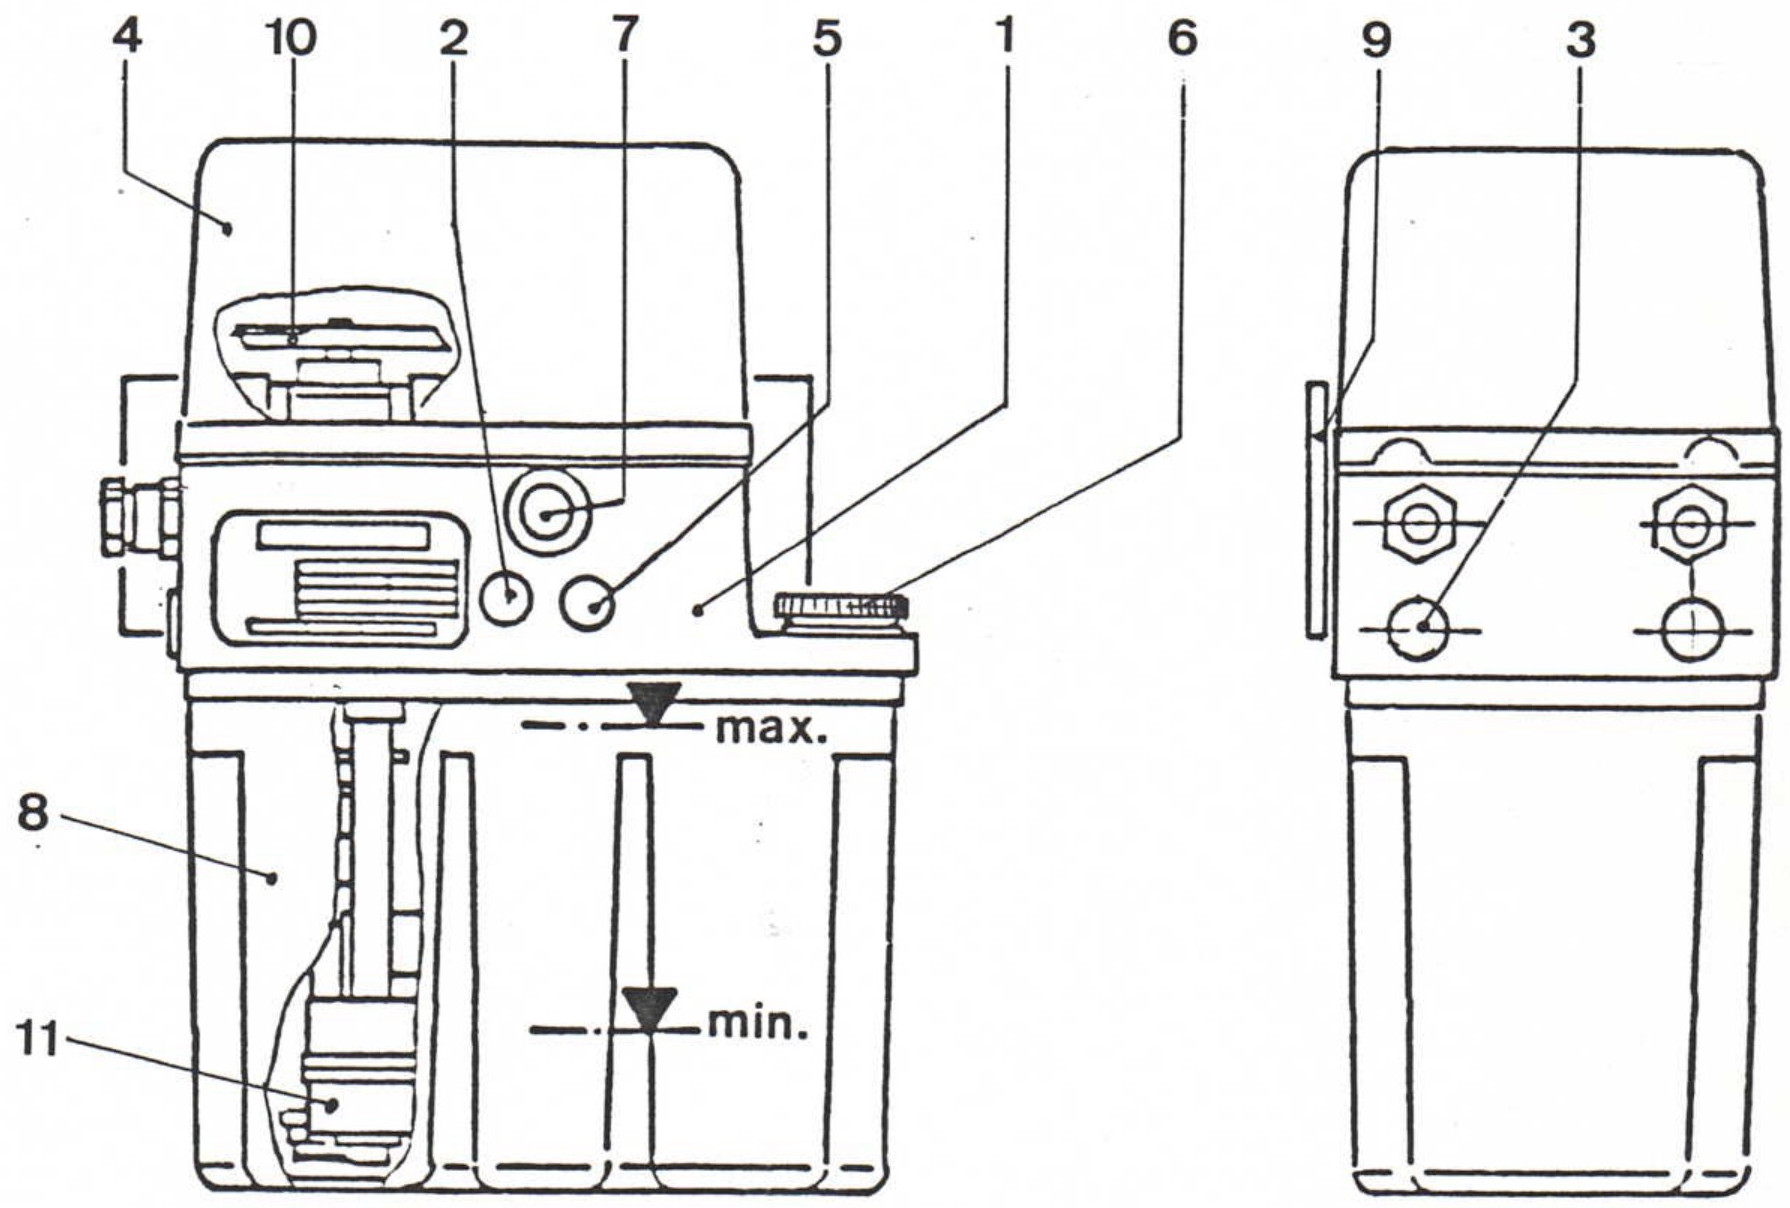
\includegraphics[width=0.8\textwidth]{images/lubrication_unit.jpg}
\end{figure}

\begin{enumerate}
    \item Central lubrication unit
    \item Green indicator light \textit{"Operation"}
    \item Pressure connection R 1/4"
    \item Cover
    \item Red indicator light \textit{"Fault"}
    \item Oil filling opening with built-in sieve
    \item Push button for manually triggering the lubrication pulse
    \item Transparent container
    \item Mounting plate
    \item Fan wheel
    \item Float switch
\end{enumerate}

\notebox{WARNING}{%
    The values set under machine constants MC 758, 759, 767, and 768 must not be changed.
}

\noindent Pump runtime until pressure build-up, plus 15 s overrun time (MC 768 = 15).

\vspace{.3cm}

\noindent A fault signal occurs if the pressure build-up fails 60 s after the pump starts.

\sectionLikeSubsection{Automatic Central Lubrication}

\subsection*{Functionality}

The motion-independent automatic central lubrication ensures an even supply of oil to all sliding surfaces and moving elements of the machine.

\vspace{.3cm}

\noindent Through a lubrication pulse, the pump of the central lubrication unit (1) starts and pumps oil into the pipeline system until the necessary pressure for oil supply is reached. Once this pressure is achieved, a pressure monitor switches the pump off.

\vspace{.3cm}

\noindent During the lubrication process, the green indicator light (2) \textit{"Operation"} is illuminated.

\vspace{.3cm}

\noindent Lubrication pulses are triggered:

\begin{enumerate}
    \item With each machine start, by pressing the illuminated push button -3SH1- on the control station.\footnotemark
    \item When the machine is running without any axis movement, after every 8 hours. (MC 767 = 480).
    \item When the movement of one or multiple axes, with or without interruptions, lasts longer than 16 minutes. (MC 758 = 16).
    \item When an axis starts moving and the last lubrication pulse was more than 32 minutes ago. (MC 759 = 32).
\end{enumerate}

\noindent If lubrication fails, the pressure monitor causes the shutdown of the hydraulics and feed drive. The red indicator light (5) \textit{"Fault"} illuminates, and the machine is automatically stopped through the emergency stop circuit.

\subsection*{Restarting the Machine after Lubrication Failure}

\begin{itemize}
    \item Check the oil level in the transparent container (8) and refill if necessary via the filling opening (6).\footnotemark
    \item Check the main line between the central lubrication unit (1) and oil distributors (see sheet 3.20-1) for leaks.
\end{itemize}

\subsection*{After Resolving the Malfunction}

\begin{itemize}
    \item Press the illuminated push button -3SH1- on the control station.\footnotemark[1]
    \item The indicator light -3H1- illuminates.
\end{itemize}

\notebox{note}{%
    After a long downtime of the machine, additional lubrication pulses can be triggered if necessary by pressing the push button (7) on the central lubrication unit. The indicator light (2) \textit{"Operation"} must light up and must turn off at the end of the lubrication process. This must be done before \textbf{"PROGRAM START"}, as otherwise, the program sequence would be interrupted by \textit{"Spindle and feed stop"}.
}

\footnotetext[1]{Arrangement and function of the control elements on the control station, see sheet 2.04-1.}
\footnotetext[2]{See sheet 7.06-1 \textit{"Lubricant Recommendations"}.}

\sectionLikeSubsection{Automatic Central Lubrication - Hydraulic Plan and Circuit Diagram}

\subsection*{Hydraulic Plan}

\begin{minipage}{0.65\textwidth}
    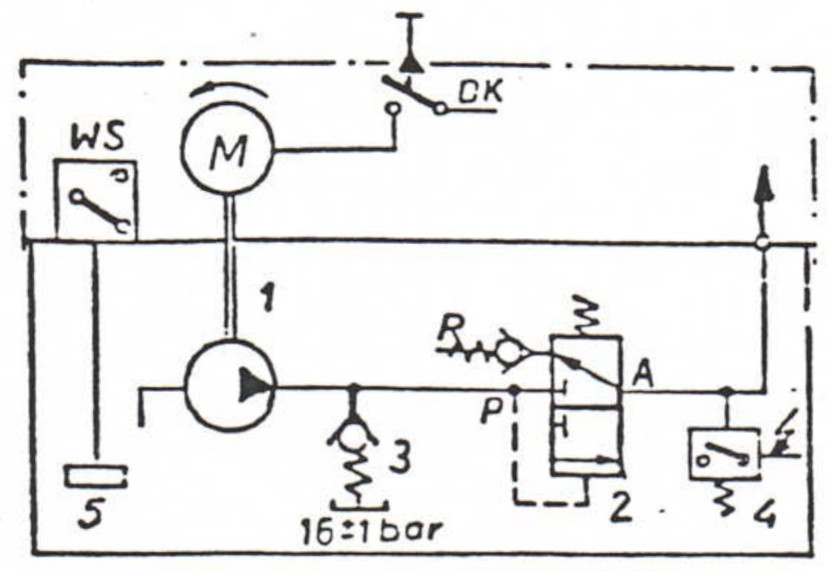
\includegraphics[width=.8\linewidth]{hydraulic_plan.jpg}
\end{minipage}%
\begin{minipage}{0.35\textwidth}
    \begin{itemize}
        \item[1] Gear Pump Unit
        \item[2] Hydraulic Valve
        \item[3] Pressure Relief Valve
        \item[4] Pressure Switch
        \item[5] Float
    \end{itemize}
    
    \vspace{1em}
    \textbf{Pump Output:} 0.1 l/min \\
    \textbf{Max Connection Volume:} 18 cm\textsuperscript{3}
\end{minipage}

\vspace{2cm}

\subsection*{Circuit Diagram (Shown for 220V)}

\begin{minipage}{0.65\textwidth}
    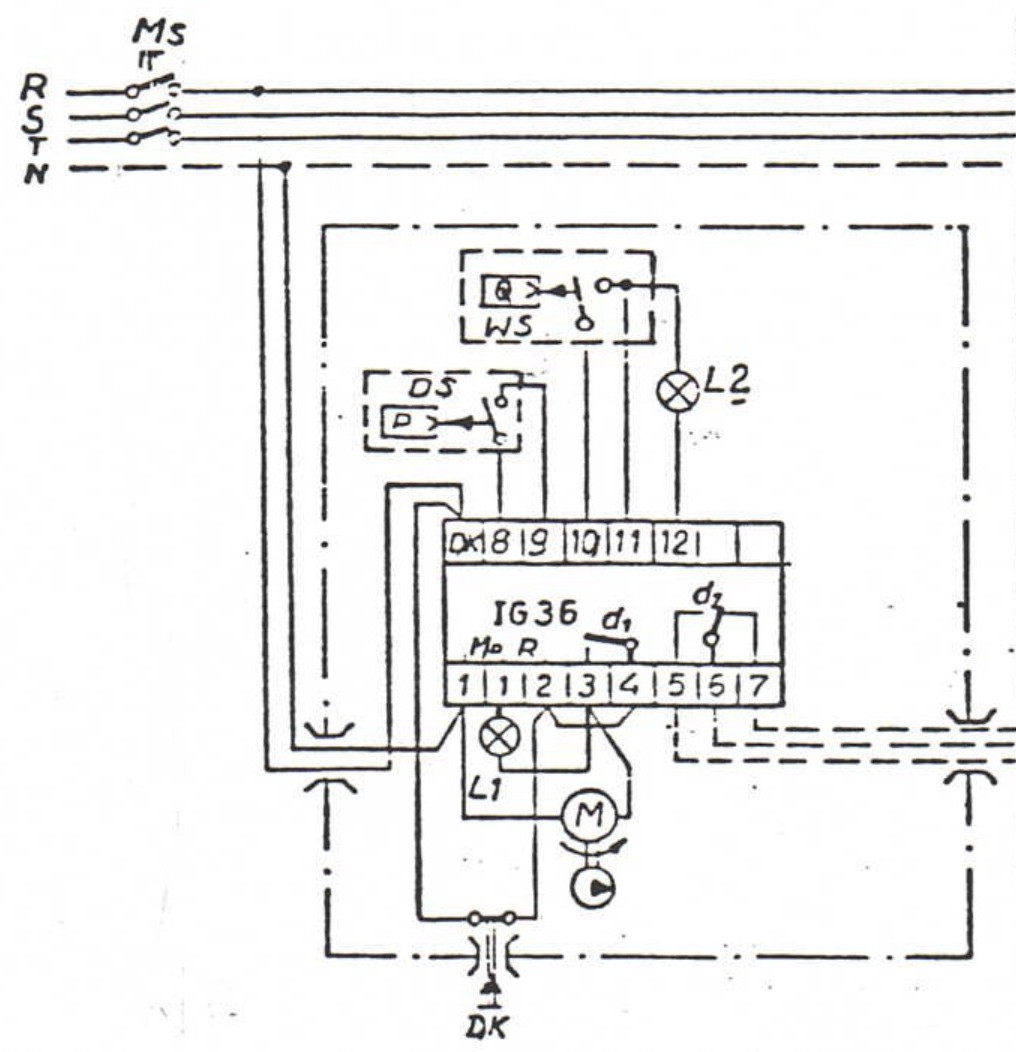
\includegraphics[width=.8\linewidth]{hydraulic_circuit_diagram.jpg}
\end{minipage}%
\begin{minipage}{0.35\textwidth}
    \begin{itemize}
        \item[\textbf{L1}] Operating Indicator Lamp 24V=
        \item[\textbf{L2}] Fault Indicator Lamp 24V=
        \item[\textbf{Ws}] Float Switch
        \item[\textbf{Ds}] Pressure Switch
        \item[\textbf{IG 36}] Control Device
        \item[\textbf{DK}] Push Button
        \item[\textbf{Ms}] Machine Main Switch
    \end{itemize}
\end{minipage}

\vspace{1cm}

\noindent
\begin{tabular}{ll}
    Total Power Consumption: & \textbf{100 W} \\
    Motor Power: & \textbf{20 W} \\
    Motor Pump Speed: & \textbf{2600 min\textsuperscript{-1}}
\end{tabular}

\section{Coolant Lubrication System}

\setcounter{section}{22}

\begin{figure}[h]
    \centering
    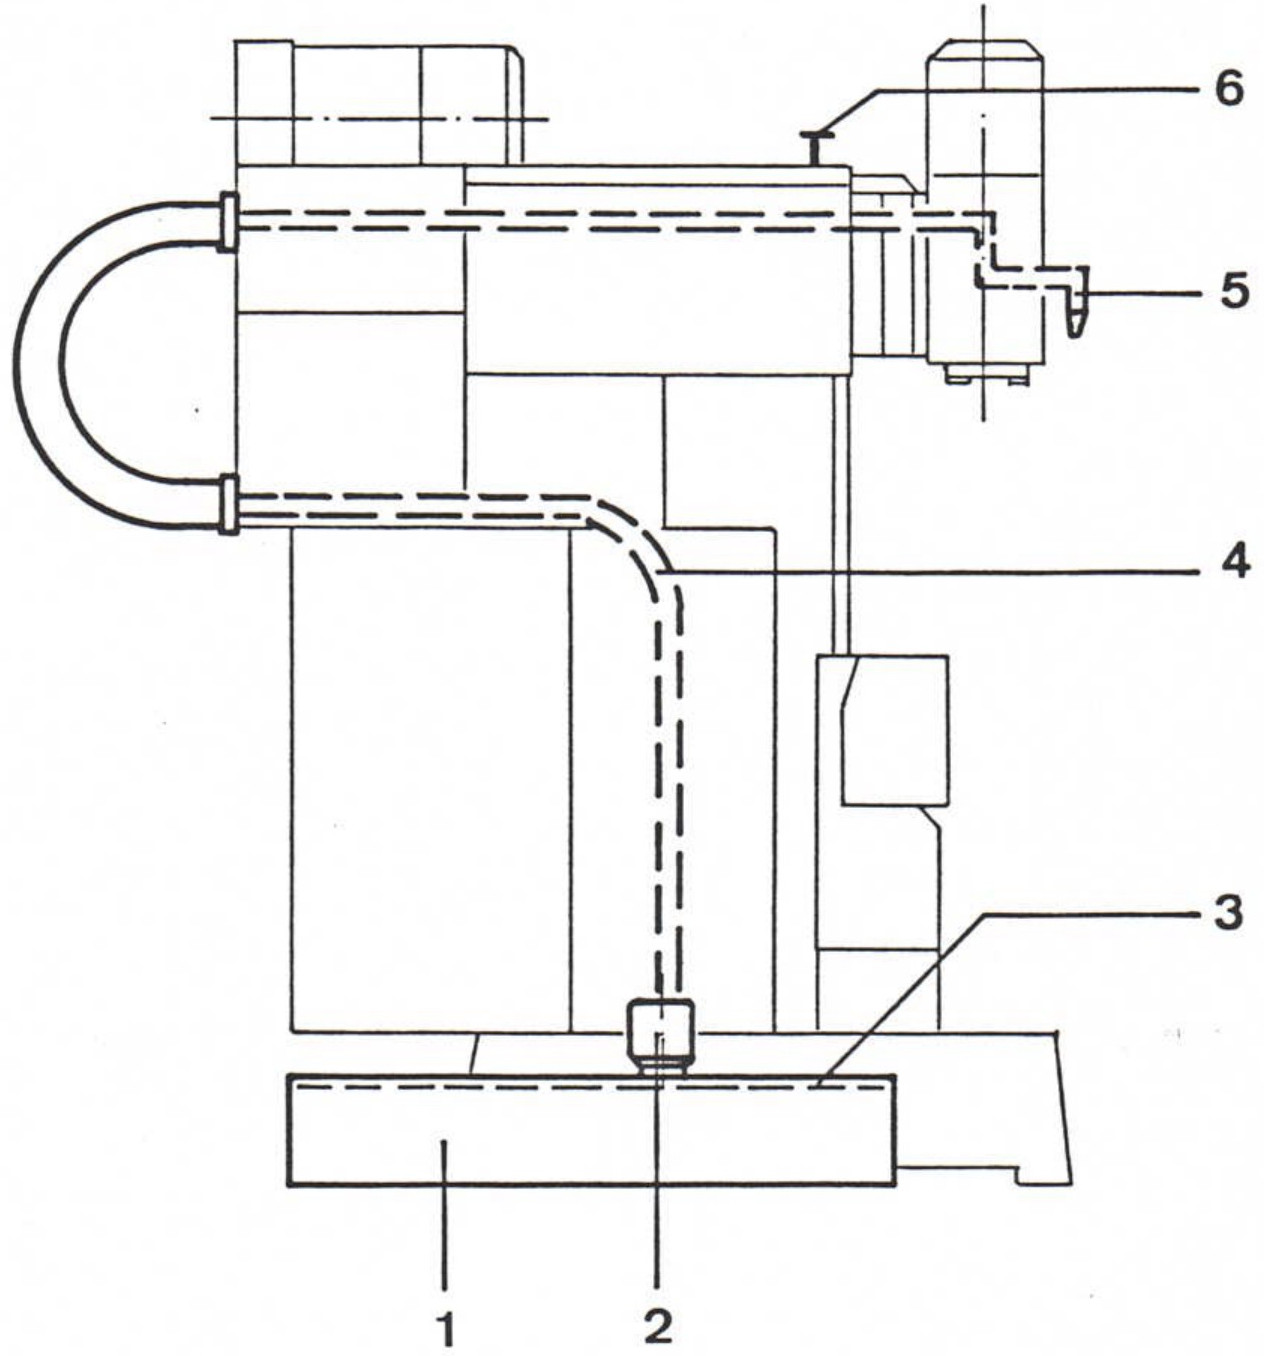
\includegraphics[width=0.8\textwidth]{coolant_system.jpg}
\end{figure}

\noindent
\begin{enumerate}
    \item Coolant reservoir (Capacity approx. 80 l)\footnotemark
    \item Coolant pump -2M1- (Flow rate 56 l/min at 2°E/50°C)\footnotemark
    \item Removable cover plate
    \item Connecting pipe between pump -2M1- and spindle head
    \item Adjustable pipe with nozzle for coolant supply to the tool\footnotemark
    \item Valve for adjusting the coolant flow
\end{enumerate}

\footnotetext[1]{To avoid foam formation, the coolant reservoir should be kept as full as possible.}
\footnotetext[2]{The coolant pump is switched on using program code \texttt{M8} and off using \texttt{M9} on the CNC control panel (see CNC manual \#32).}
\footnotetext[3]{For coolant specifications, see sheet 7.07-1.}

\section{Splash Protection}

\setcounter{section}{24}

The splash protection consists of a chip tray (6), which is firmly attached to the vertical clamping table and moves along the X-axis.

\begin{itemize}
    \item Two frames with safety glass (4) are attached to this chip tray (6) using hinges and can be folded down. They are connected by locks (2). The right side panel (5) can be unfolded and lowered.
    \item The rear splash guard (3) is fixed to the cross support and moves along the Y-axis.
    \item When switching from horizontal to vertical machining, the flap (1) is opened.
\end{itemize}

\notebox{Warning}{The reconfiguration may only be performed in the position \texttt{+Y 370 / -X 75} of the cross support. When not in use, the vertical milling head must be precisely fixed in its resting position (see Sheet 3.07-1 / 3.08-1).}

\noindent To empty the chip tray, the bottom flap (7) must be opened using a control cabinet key. The screens in the table and the chip tray should be cleaned as needed. Use only household cleaning agents to clean the safety glass panes.

\vspace{.5cm}

\notebox{Warning}{When using a swiveled milling head, operation is only possible with a reduced X-axis travel to avoid collision hazards.}

\begin{figure}[h]
    \centering
    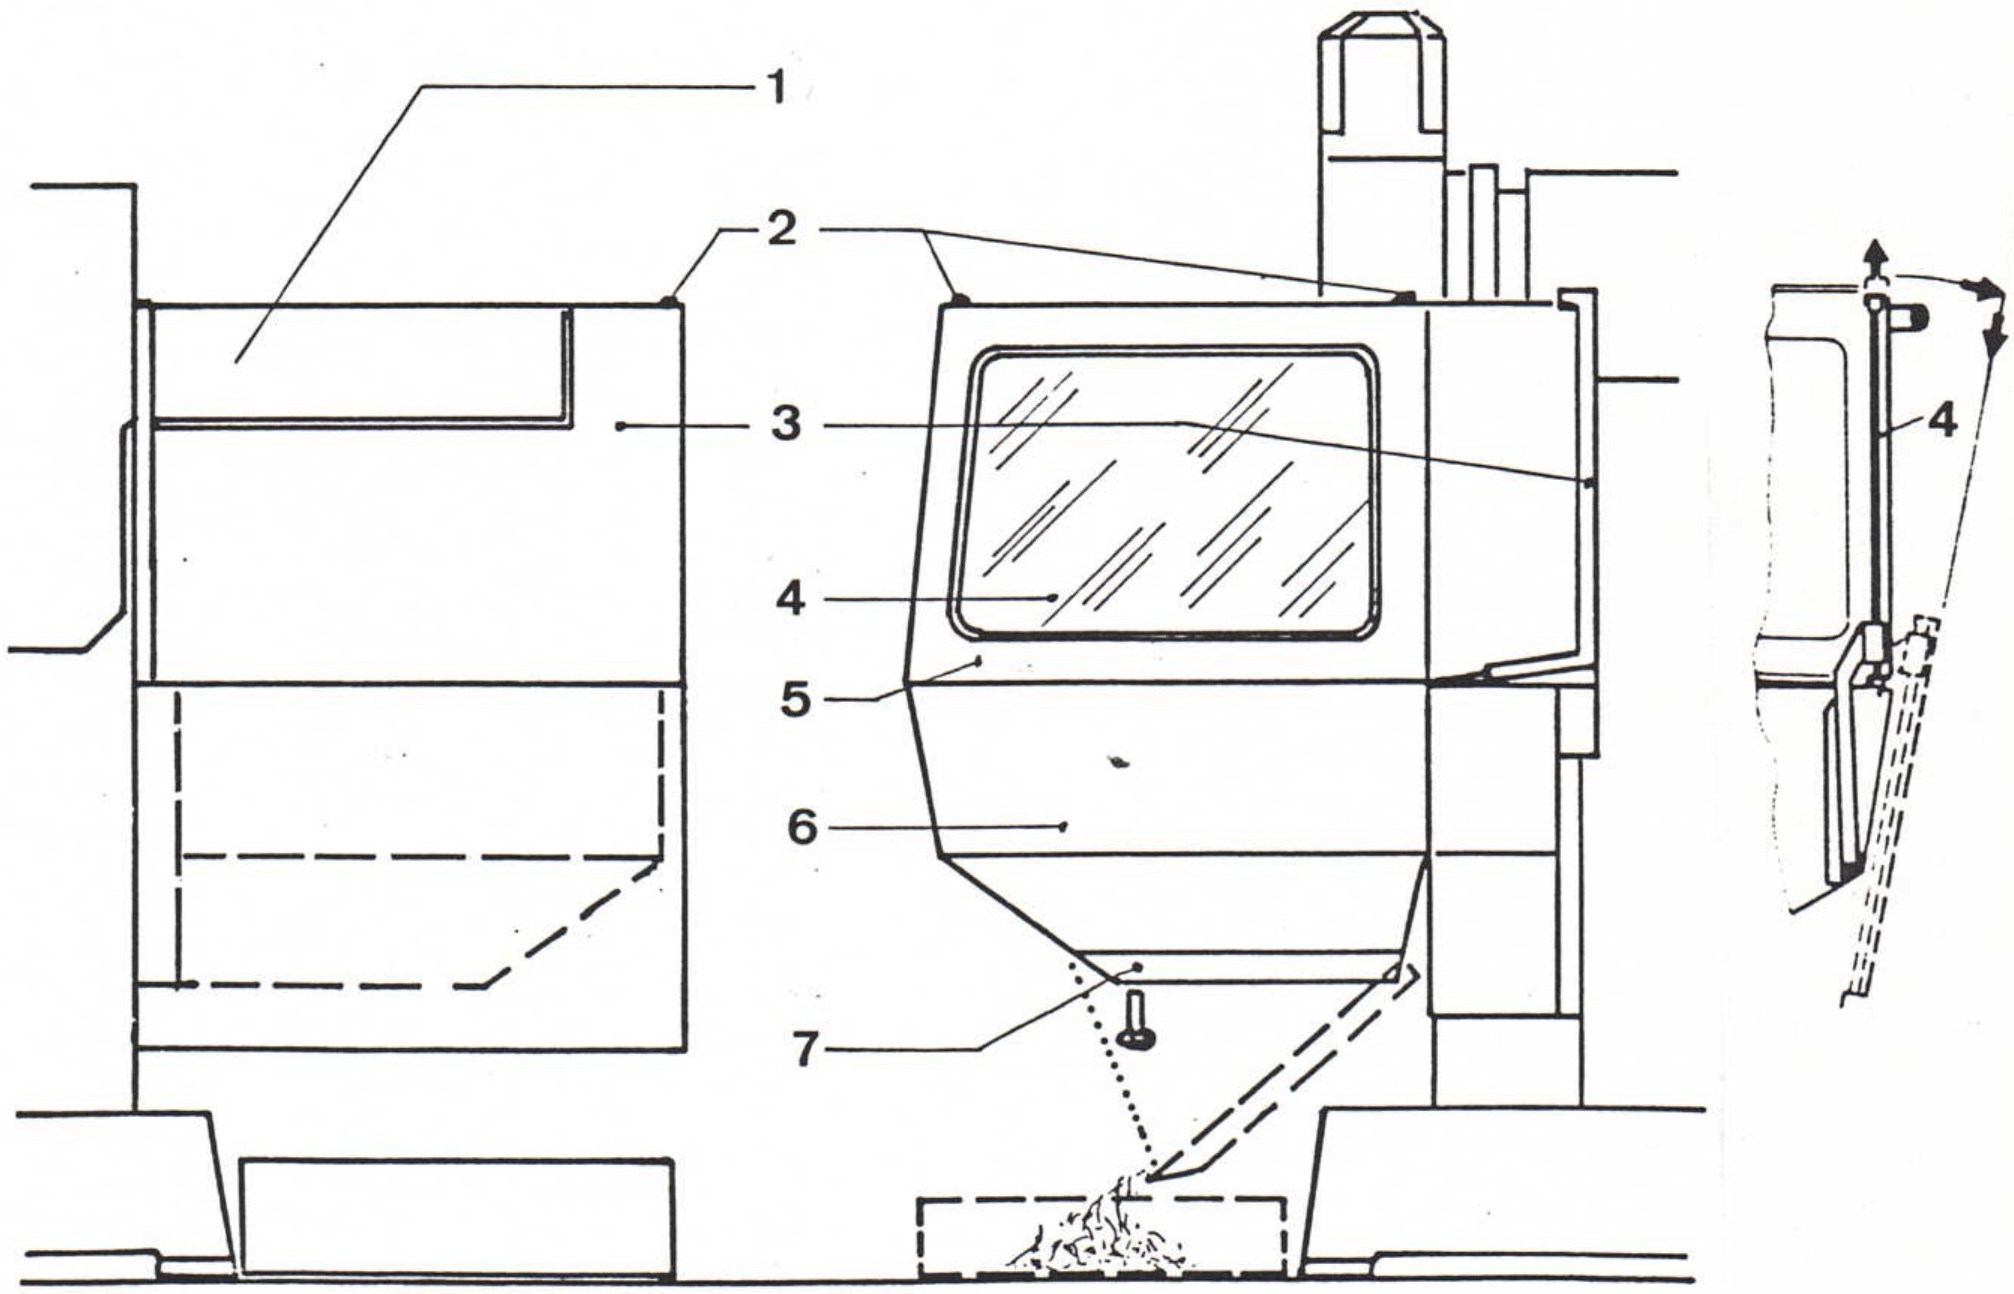
\includegraphics[width=\textwidth]{splash_protection.jpg}
\end{figure}
